\chapter{Eksperymenty i wyniki}

W rozdziale przedstawiono zmiany interfejsu i funkcjonalności aplikacji wprowadzone w celu poprawy doświadczenia użytkownika oraz wyniki badań modelu wykrywania wydechu. Porównano ekrany przed modyfikacjami, a także po ich wdrożeniu, a następnie przeanalizowano skuteczność modeli BCV2 i BCV3 oraz dobór progu decyzyjnego w różnych konfiguracjach sprzętowych.

\section{Badania związane z UX/UI}

Prace nad interfejsem obejmowały przegląd treningu, sposób prezentowania ćwiczeń, edycję etapów, ustawienia dźwięku i konfigurację detekcji wydechu. Celem zmian było zwiększenie czytelności ekranów oraz rozszerzenie możliwości dostosowania treningu do preferencji użytkownika. Poniższe zestawienia dokumentują zakres wprowadzonych usprawnień. Mają charakter porównania funkcjonalnego, jak również wizualnego.

\subsection{Usprawnienie ekranu przeglądu treningu}

Ekran przeglądu treningu rozszerzono o prezentację podziału etapów na grupy. Użytkownik może przed rozpoczęciem ćwiczenia sprawdzić kolejność grup, należące do nich etapy oraz liczbę powtórzeń. Wyróżnienie grup kolorami ułatwia odczytanie struktury treningu, zwłaszcza gdy obejmuje on kilka różnych sekwencji oddechowych.


Dodatkowo przyrost czasu trwania jest przedstawiany osobno dla każdej fazy, gdzie w poprzednich wersjach nie był on wyświetlany w ogóle. Sposób prezentacji wynika z wprowadzonej w edytorze treningu możliwości niezależnego dostosowywania przyrostu dla poszczególnych faz. Widoczne wartości odzwierciedlają ustawienia wybrane podczas edycji i pozwalają użytkownikowi sprawdzić je przed rozpoczęciem ćwiczenia. Porównanie obu wersji ekranu przedstawiono na rysunku \ref{fig:ux_training_overview}.

\begin{figure}[H]
    \centering
    \begin{minipage}[c]{0.44\linewidth}
        \centering
        {\setlength{\fboxsep}{0pt}\setlength{\fboxrule}{0.2pt}\fcolorbox{gray}{white}{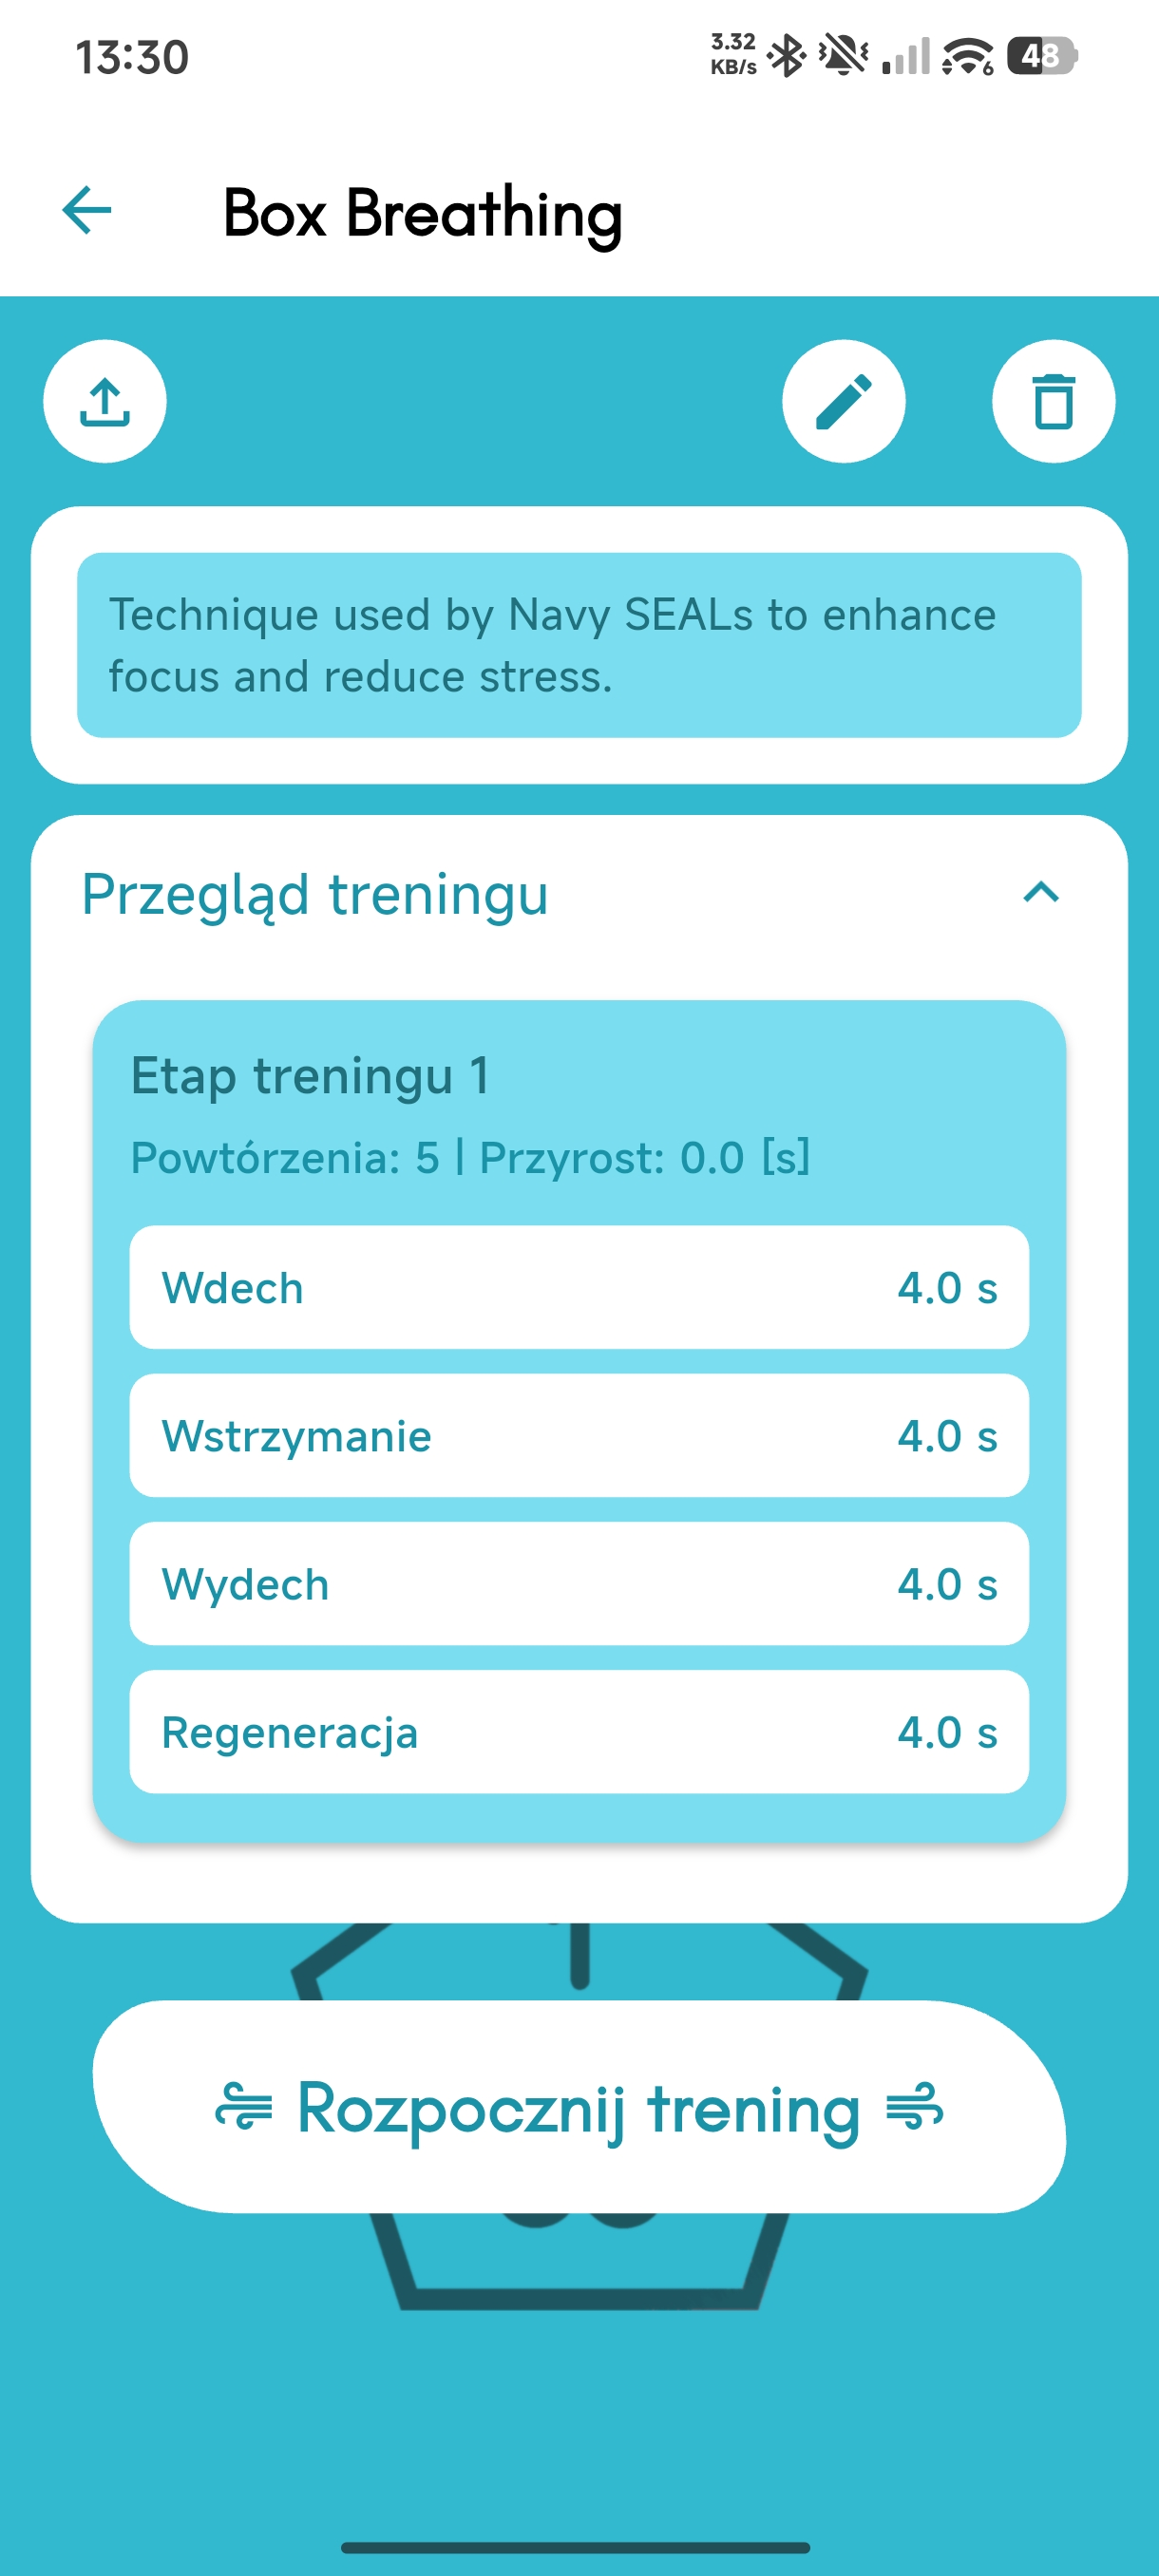
\includegraphics[width=\dimexpr\linewidth-2\fboxrule\relax,height=0.64\textheight,keepaspectratio]{obrazy/badania_interface/start_menu_old.jpg}}}
        \par\small (a)
    \end{minipage}\hfill
    \begin{minipage}[c]{0.08\linewidth}
        \centering
        {\large $\rightarrow$}
    \end{minipage}\hfill
    \begin{minipage}[c]{0.44\linewidth}
        \centering
        {\setlength{\fboxsep}{0pt}\setlength{\fboxrule}{0.2pt}\fcolorbox{gray}{white}{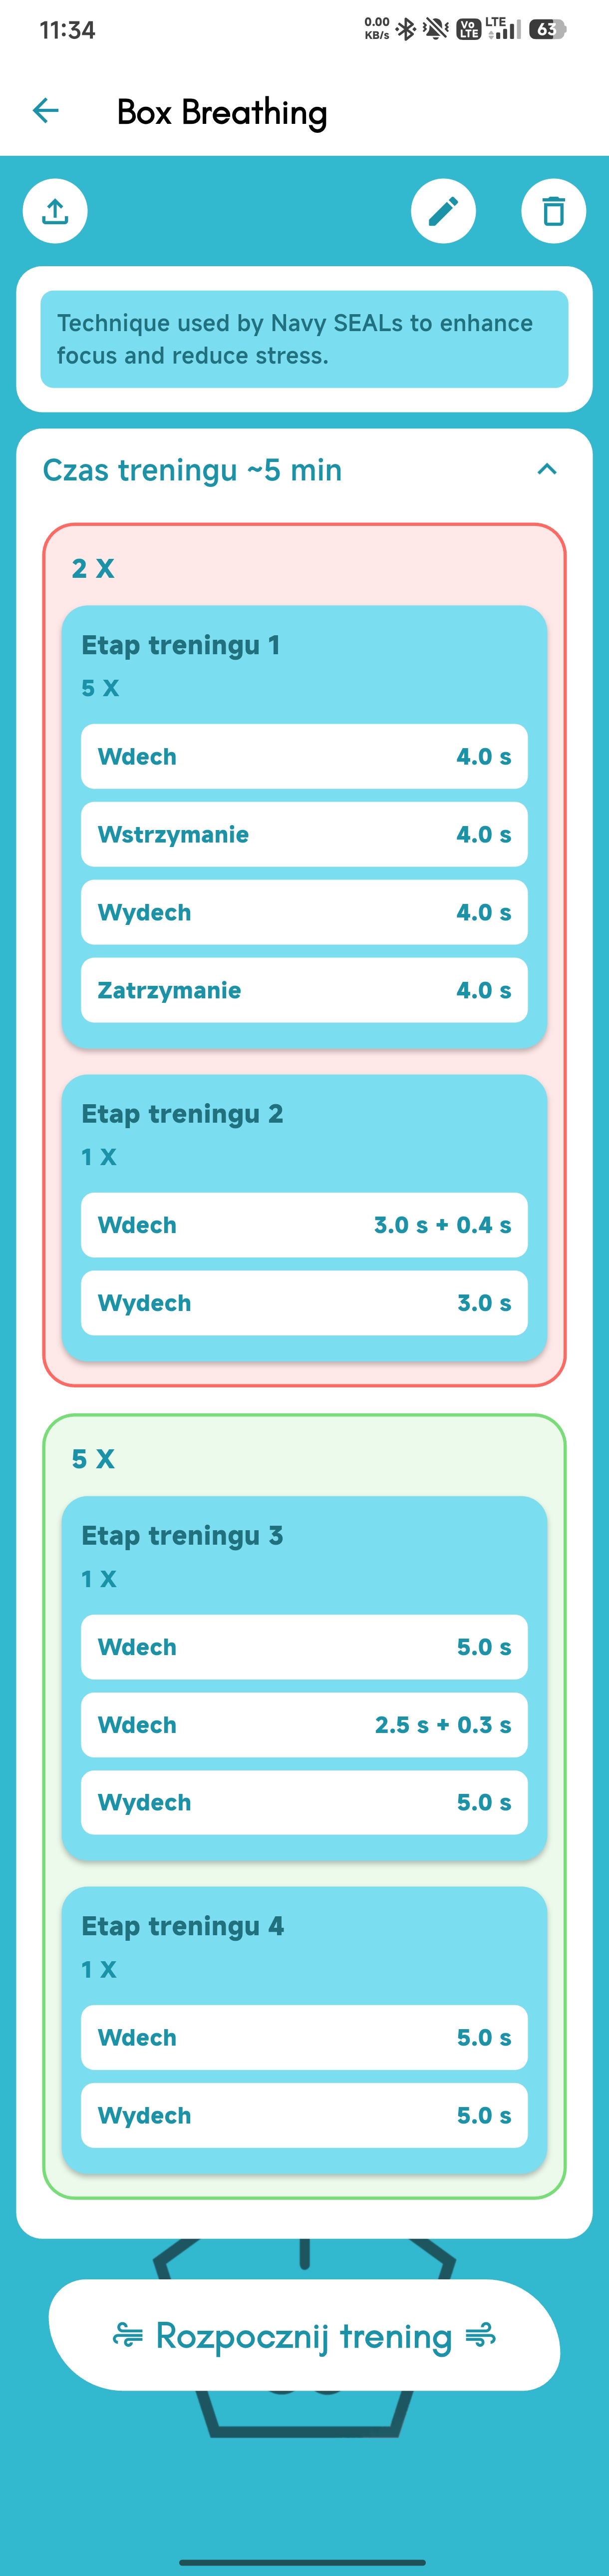
\includegraphics[width=\dimexpr\linewidth-2\fboxrule\relax,height=0.64\textheight,keepaspectratio]{obrazy/badania_interface/start_menu_new.jpg}}}
        \par\small (b)
    \end{minipage}
    \caption[Przegląd treningu przed zmianami i po rozbudowie]{Przegląd treningu: (a) ekran przed zmianami; (b) ekran po dodaniu grup oraz indywidualnych przyrostów czasu faz}
    \label{fig:ux_training_overview}
\end{figure}

\subsection{Ekran treningu oddechowego}
\label{sec:ux_breathing_visualization}

W pierwotnej wersji aplikacji przebieg treningu przedstawiano za pomocą pulsujących okręgów. Dodano alternatywną wizualizację w postaci fali na osi czasu, która pokazuje przebieg kolejnych faz oddechu. Wybór ten nawiązuje do omówionego wcześniej artykułu \textit{Evaluating mobile apps for breathing training: The effectiveness of visualization} \cite{chittaro2014evaluating}, w którym użytkownicy preferowali wizualizację falową. W odróżnieniu od kuli lub okręgu fala pozwala przedstawić także nadchodzące fazy, co było przesłanką do udostępnienia tego wariantu w aplikacji. Wyników przywołanego badania nie należy jednak utożsamiać z pomiarem skuteczności interfejsu ReSpire.

Trening można również realizować, korzystając wyłącznie ze wskazówek dźwiękowych, bez potrzeby obserwowania ekranu. Dostępne są komunikaty lektora oraz sonifikacja, czyli dźwięk narastający i opadający zgodnie z przebiegiem oddechu. Rozszerzenie to umożliwia wybór sposobu prowadzenia ćwiczenia odpowiadającego preferencjom użytkownika.

Dodano ponadto możliwość zaplanowania dwóch szybkich wdechów następujących bezpośrednio po sobie. Funkcja odpowiada na wskazaną potrzebę użytkowników i rozszerza zakres możliwych do skonfigurowania sekwencji faz oddechu. Na rysunku \ref{fig:ux_breathing_views} zestawiono pierwotną wizualizację, widok fali oraz przykład dwóch kolejnych wdechów.

\begin{figure}[H]
    \centering
    \begin{minipage}[c]{0.29\linewidth}
        \centering
        {\setlength{\fboxsep}{0pt}\setlength{\fboxrule}{0.2pt}\fcolorbox{gray}{white}{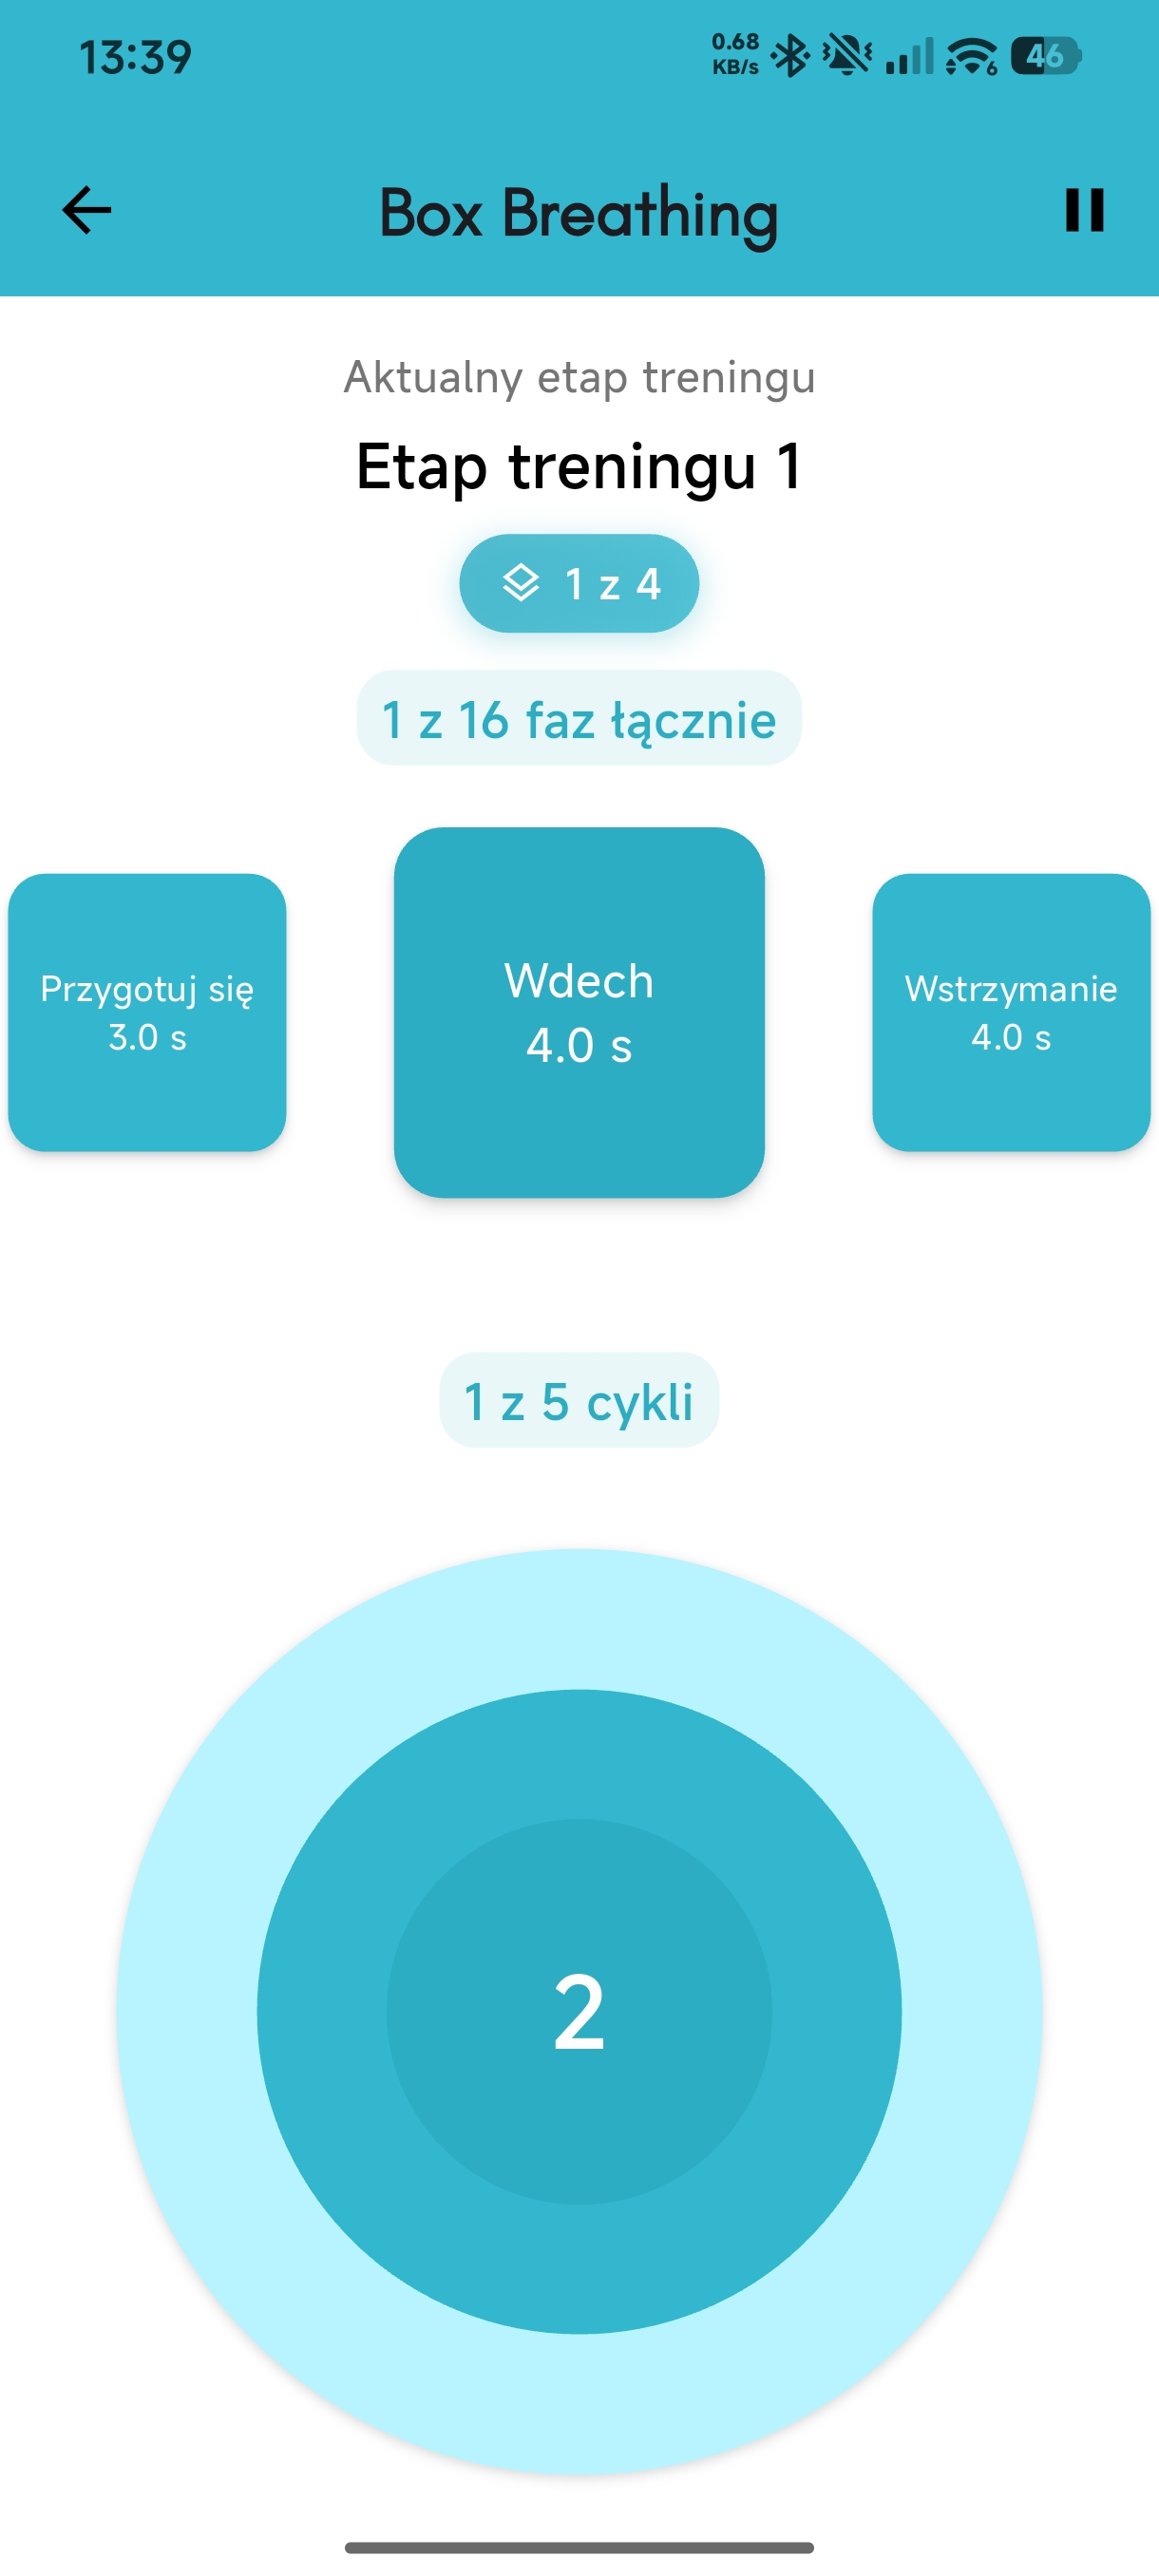
\includegraphics[width=\dimexpr\linewidth-2\fboxrule\relax]{obrazy/badania_interface/breathing_page_ring_old.jpg}}}
        \par\small (a)
    \end{minipage}\hfill
    \begin{minipage}[c]{0.06\linewidth}
        \centering
        {\large $\rightarrow$}
    \end{minipage}\hfill
    \begin{minipage}[c]{0.29\linewidth}
        \centering
        {\setlength{\fboxsep}{0pt}\setlength{\fboxrule}{0.2pt}\fcolorbox{gray}{white}{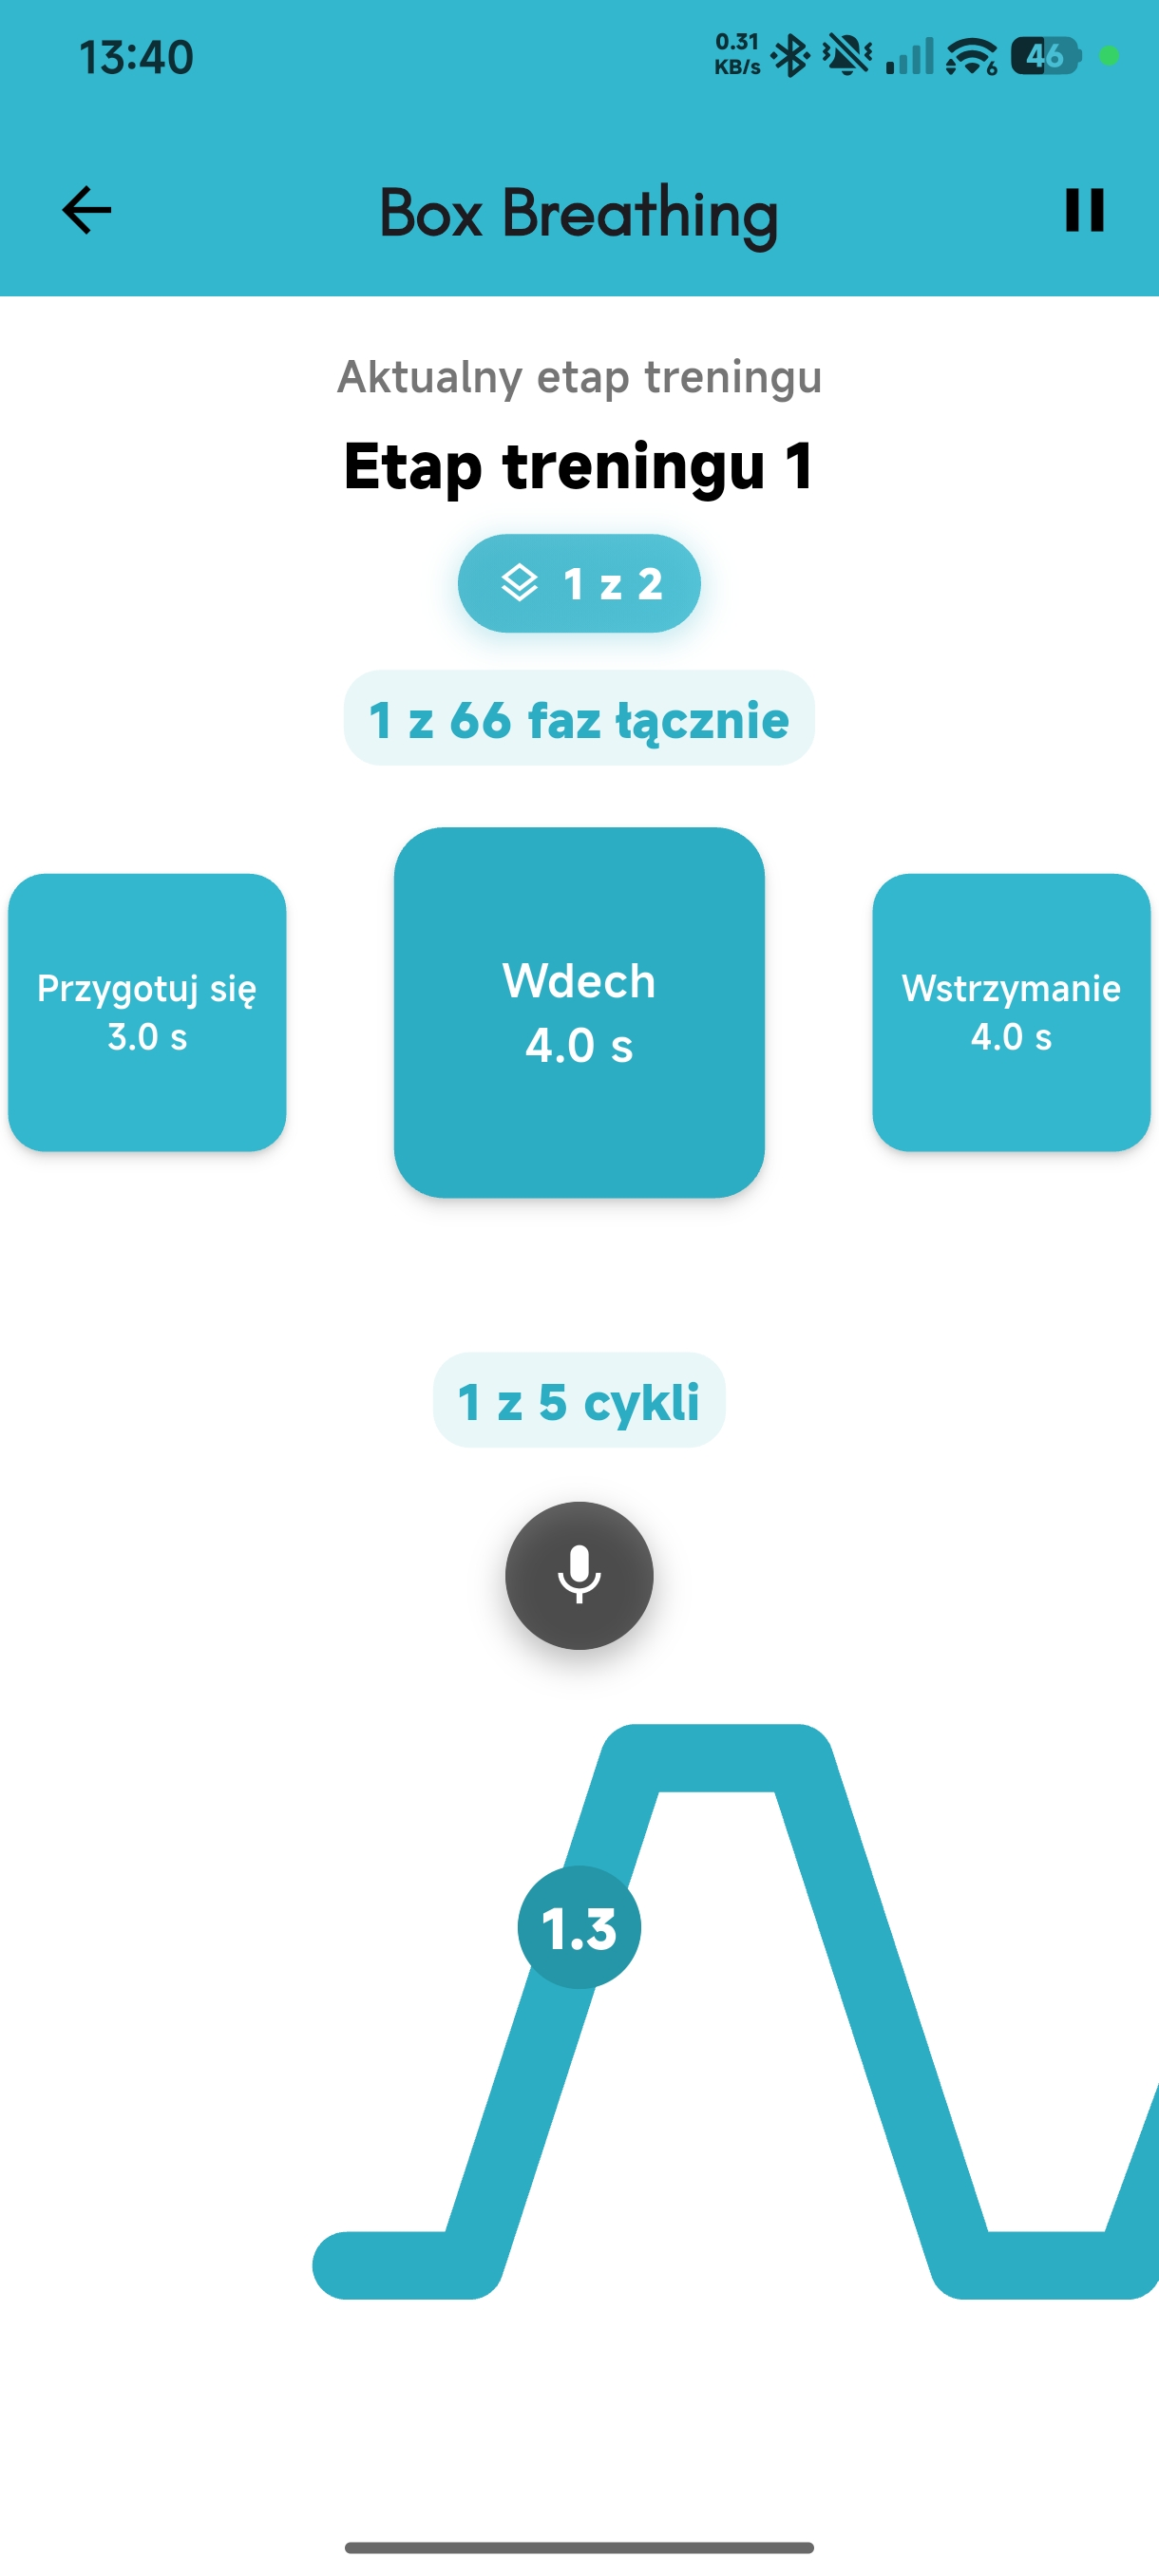
\includegraphics[width=\dimexpr\linewidth-2\fboxrule\relax]{obrazy/badania_interface/breathing_page_wave_new.jpg}}}
        \par\small (b1)
    \end{minipage}\hfill
    \begin{minipage}[c]{0.29\linewidth}
        \centering
        {\setlength{\fboxsep}{0pt}\setlength{\fboxrule}{0.2pt}\fcolorbox{gray}{white}{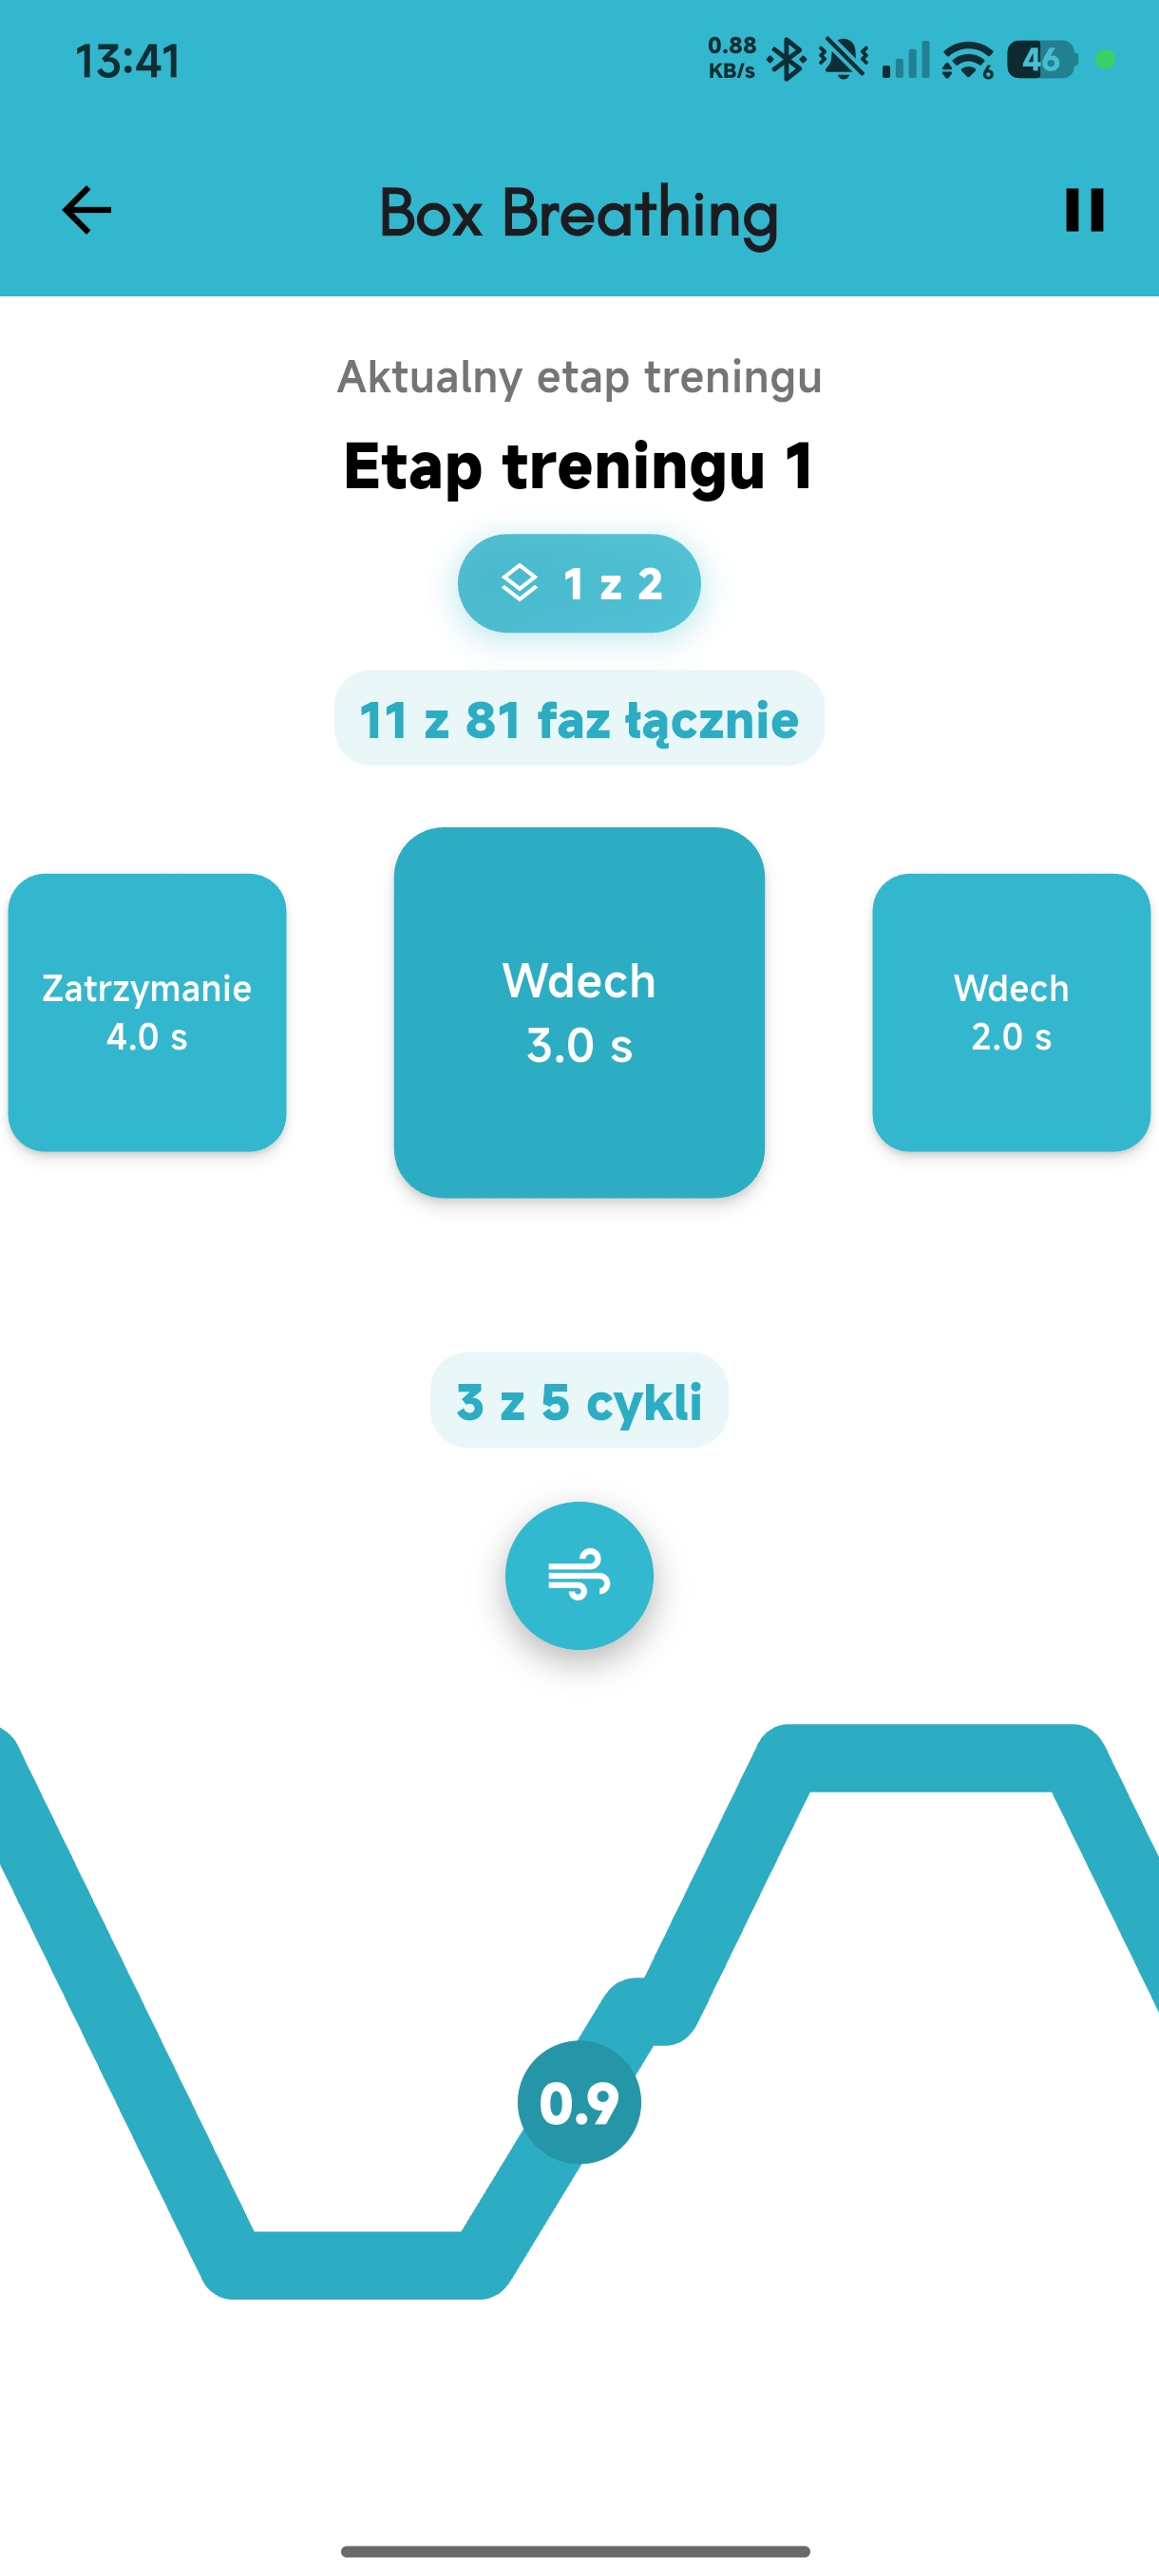
\includegraphics[width=\dimexpr\linewidth-2\fboxrule\relax]{obrazy/badania_interface/breathing_page_doube_inhale_new.jpg}}}
        \par\small (b2)
    \end{minipage}
    \caption[Porównanie sposobów wizualizacji treningu]{Wizualizacja treningu: (a) pierwotny widok okręgów; (b1) nowy widok fali; (b2) widok fali dla sekwencji dwóch kolejnych wdechów}
    \label{fig:ux_breathing_views}
\end{figure}

\subsection{Ekran edycji treningu}

Edytor rozszerzono o możliwość grupowania etapów, a także ustalania liczby powtórzeń dla konkretnej grupy. Etapy należące do danej grupy są wykonywane zgodnie z ustaloną liczbą powtórzeń przed przejściem do kolejnej grupy. Pozwala to tworzyć treningi o bardziej złożonej strukturze bez ręcznego powielania tych samych etapów. Grupy wyróżniono kolorami, a po ich utworzeniu mogą być one edytowane, łączone oraz rozdzielane.

Poprawiono również czytelność pól i etykiet, eliminując przycinanie napisów widoczne w~poprzedniej wersji. W górnej części ekranu umieszczono przybliżony czas treningu, wyznaczany na podstawie sumy czasów wszystkich zaplanowanych faz, z uwzględnieniem powtórzeń oraz zadanych przyrostów. Informacja ta umożliwia ocenę długości sesji już podczas jej konfigurowania. Na rysunku \ref{fig:ux_training_editor} przedstawiono poprzedni ekran i kolejne fragmenty rozbudowanego edytora.

\begin{figure}[H]
    \centering
    \begin{minipage}{0.31\linewidth}
        \centering
        {\setlength{\fboxsep}{0pt}\setlength{\fboxrule}{0.2pt}\fcolorbox{gray}{white}{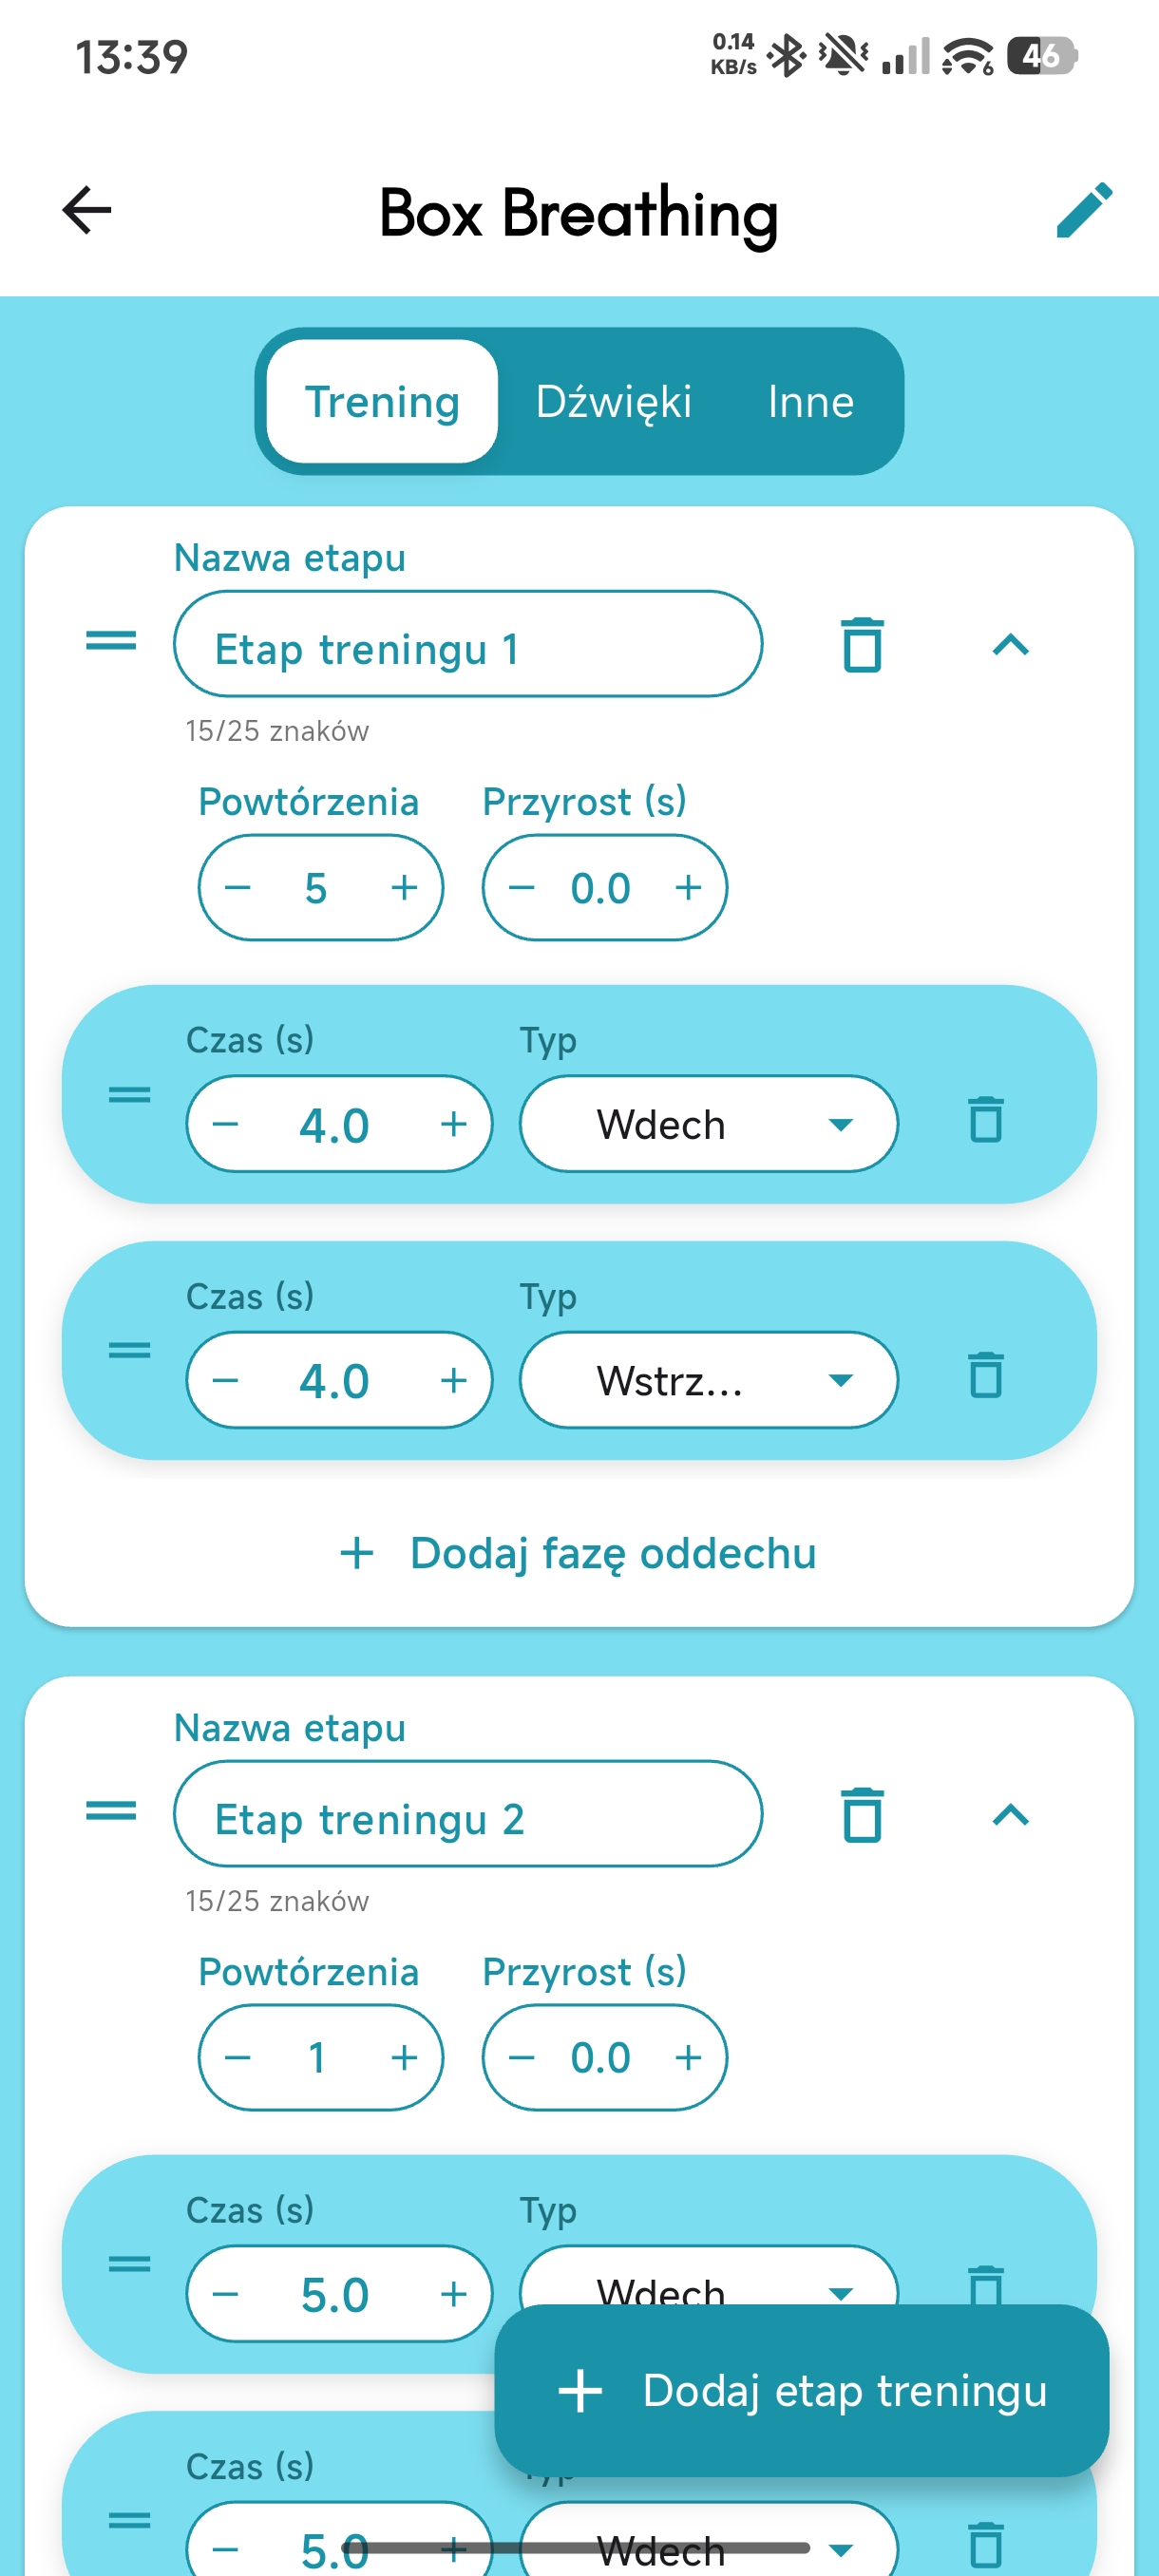
\includegraphics[width=\dimexpr\linewidth-2\fboxrule\relax]{obrazy/badania_interface/trening_edit_old.jpg}}}
        \par\small (a)
    \end{minipage}
    \par\vspace{1pt}
    {\large $\downarrow$}\par
    \vspace{1pt}
    \begin{minipage}[t]{0.31\linewidth}
        \centering
        {\setlength{\fboxsep}{0pt}\setlength{\fboxrule}{0.2pt}\fcolorbox{gray}{white}{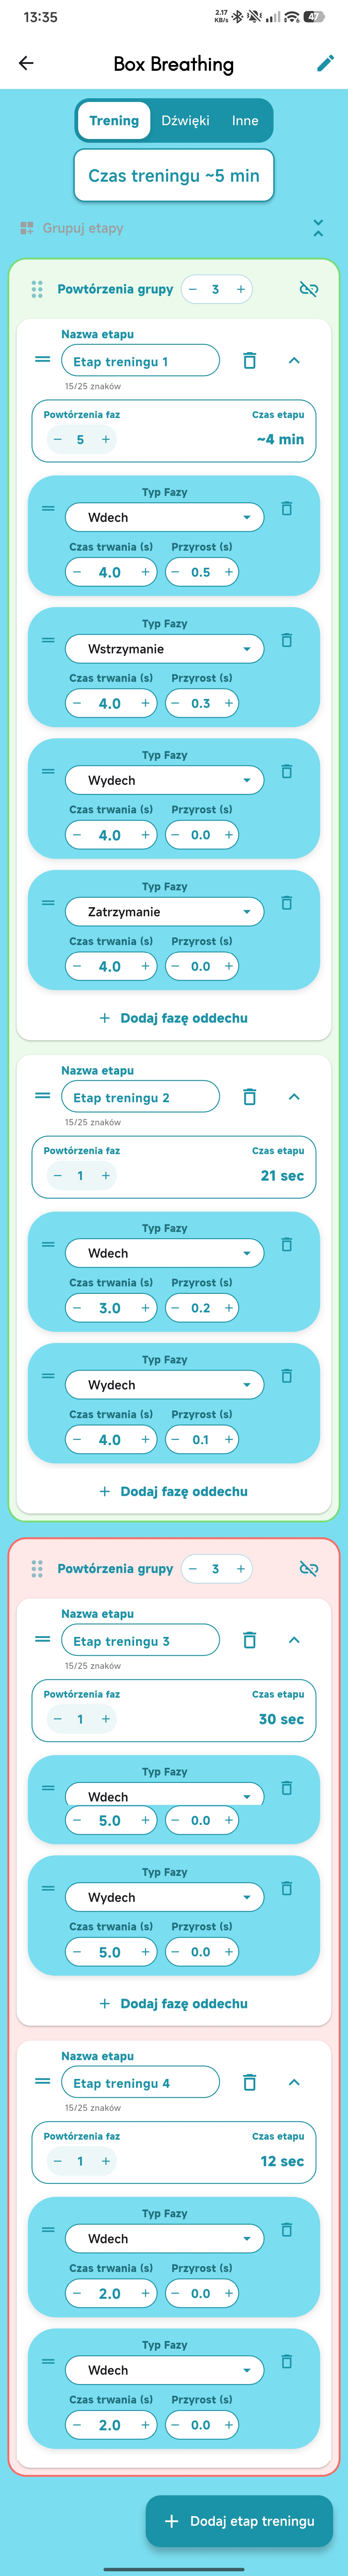
\includegraphics[width=\dimexpr\linewidth-2\fboxrule\relax,trim={0 6022bp 0 0},clip]{obrazy/badania_interface/trening_edit_new.jpg}}}
        \par\small (b1)
    \end{minipage}\hfill
    \begin{minipage}[t]{0.31\linewidth}
        \centering
        {\setlength{\fboxsep}{0pt}\setlength{\fboxrule}{0.2pt}\fcolorbox{gray}{white}{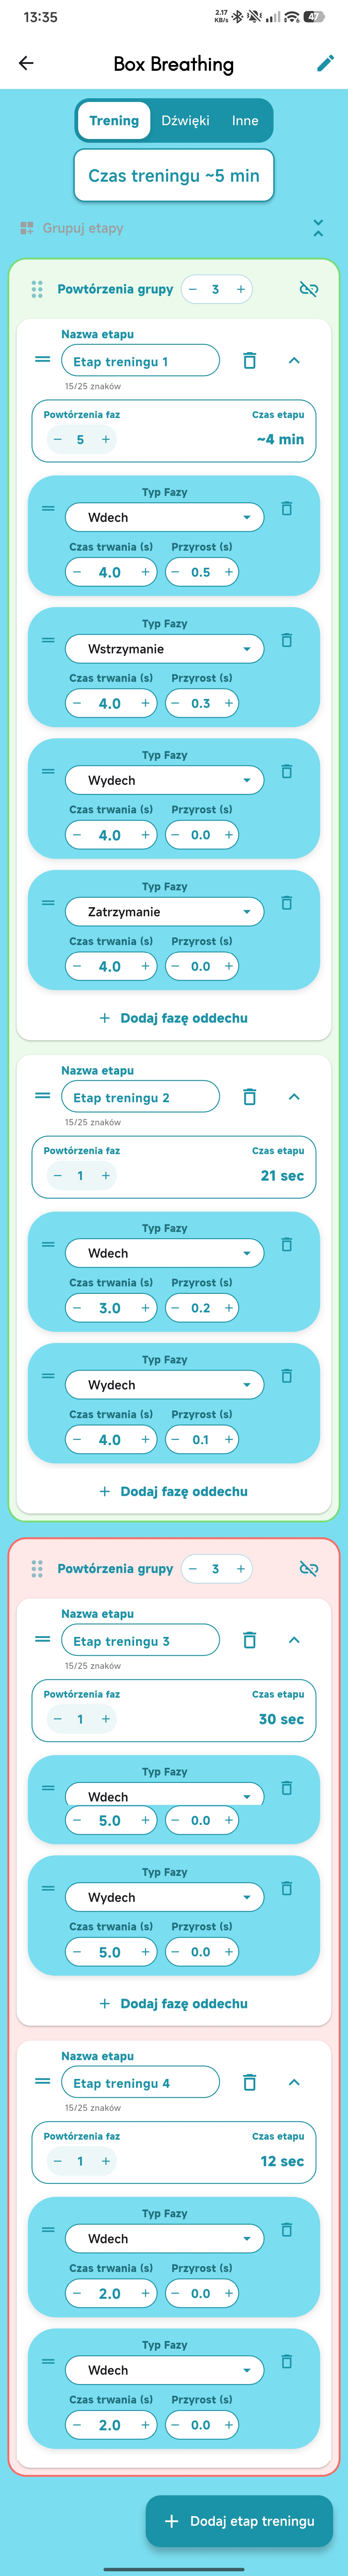
\includegraphics[width=\dimexpr\linewidth-2\fboxrule\relax,trim={0 3011bp 0 3011bp},clip]{obrazy/badania_interface/trening_edit_new.jpg}}}
        \par\small (b2)
    \end{minipage}\hfill
    \begin{minipage}[t]{0.31\linewidth}
        \centering
        {\setlength{\fboxsep}{0pt}\setlength{\fboxrule}{0.2pt}\fcolorbox{gray}{white}{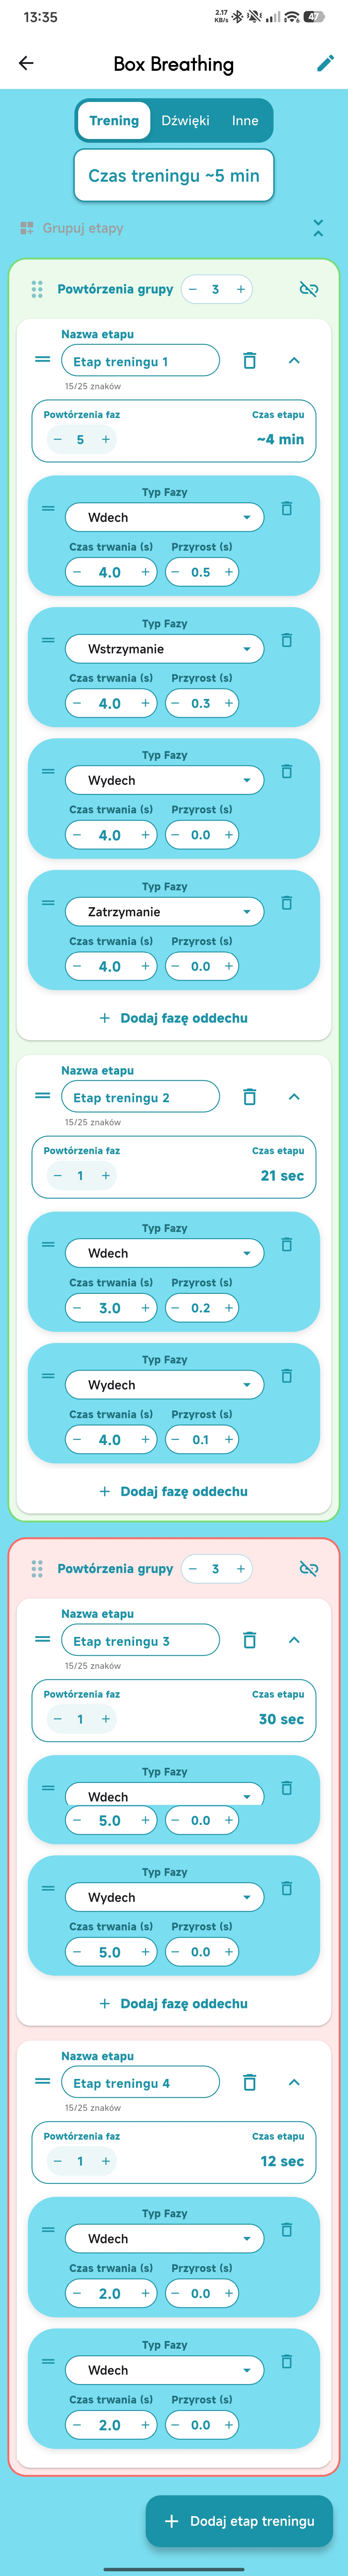
\includegraphics[width=\dimexpr\linewidth-2\fboxrule\relax,trim={0 0 0 6022bp},clip]{obrazy/badania_interface/trening_edit_new.jpg}}}
        \par\small (b3)
    \end{minipage}
    \caption[Edycja treningu przed zmianami i po rozbudowie interfejsu]{Edycja treningu: (a) ekran przed zmianami; (b1) górna część nowego ekranu z czasem treningu i ustawieniami grupy; (b2) środkowa część z kolejnymi etapami i podziałem na grupy; (b3) dolna część z ustawieniami faz oraz przyciskiem dodawania etapu}
    \label{fig:ux_training_editor}
\end{figure}

\subsection{Ekran edycji dźwięku}

W ustawieniach dźwięku ujednolicono styl komponentów, tak aby pola wyboru, suwaki i~przyciski tworzyły spójny interfejs. Ustawienia dźwięków rozpoczęcia oraz zakończenia treningu przeniesiono do zakładki \textit{Inne}, w której znajdują się również parametry czasowe tych części sesji. Rozszerzono ponadto zestaw dostępnych dźwięków. Porównanie ustawień muzyki, a także sygnałów treningowych przedstawiono na rysunku \ref{fig:ux_music_settings}.

\begin{figure}[H]
    \centering
    \begin{minipage}[c]{0.44\linewidth}
        \centering
        {\setlength{\fboxsep}{0pt}\setlength{\fboxrule}{0.2pt}\fcolorbox{gray}{white}{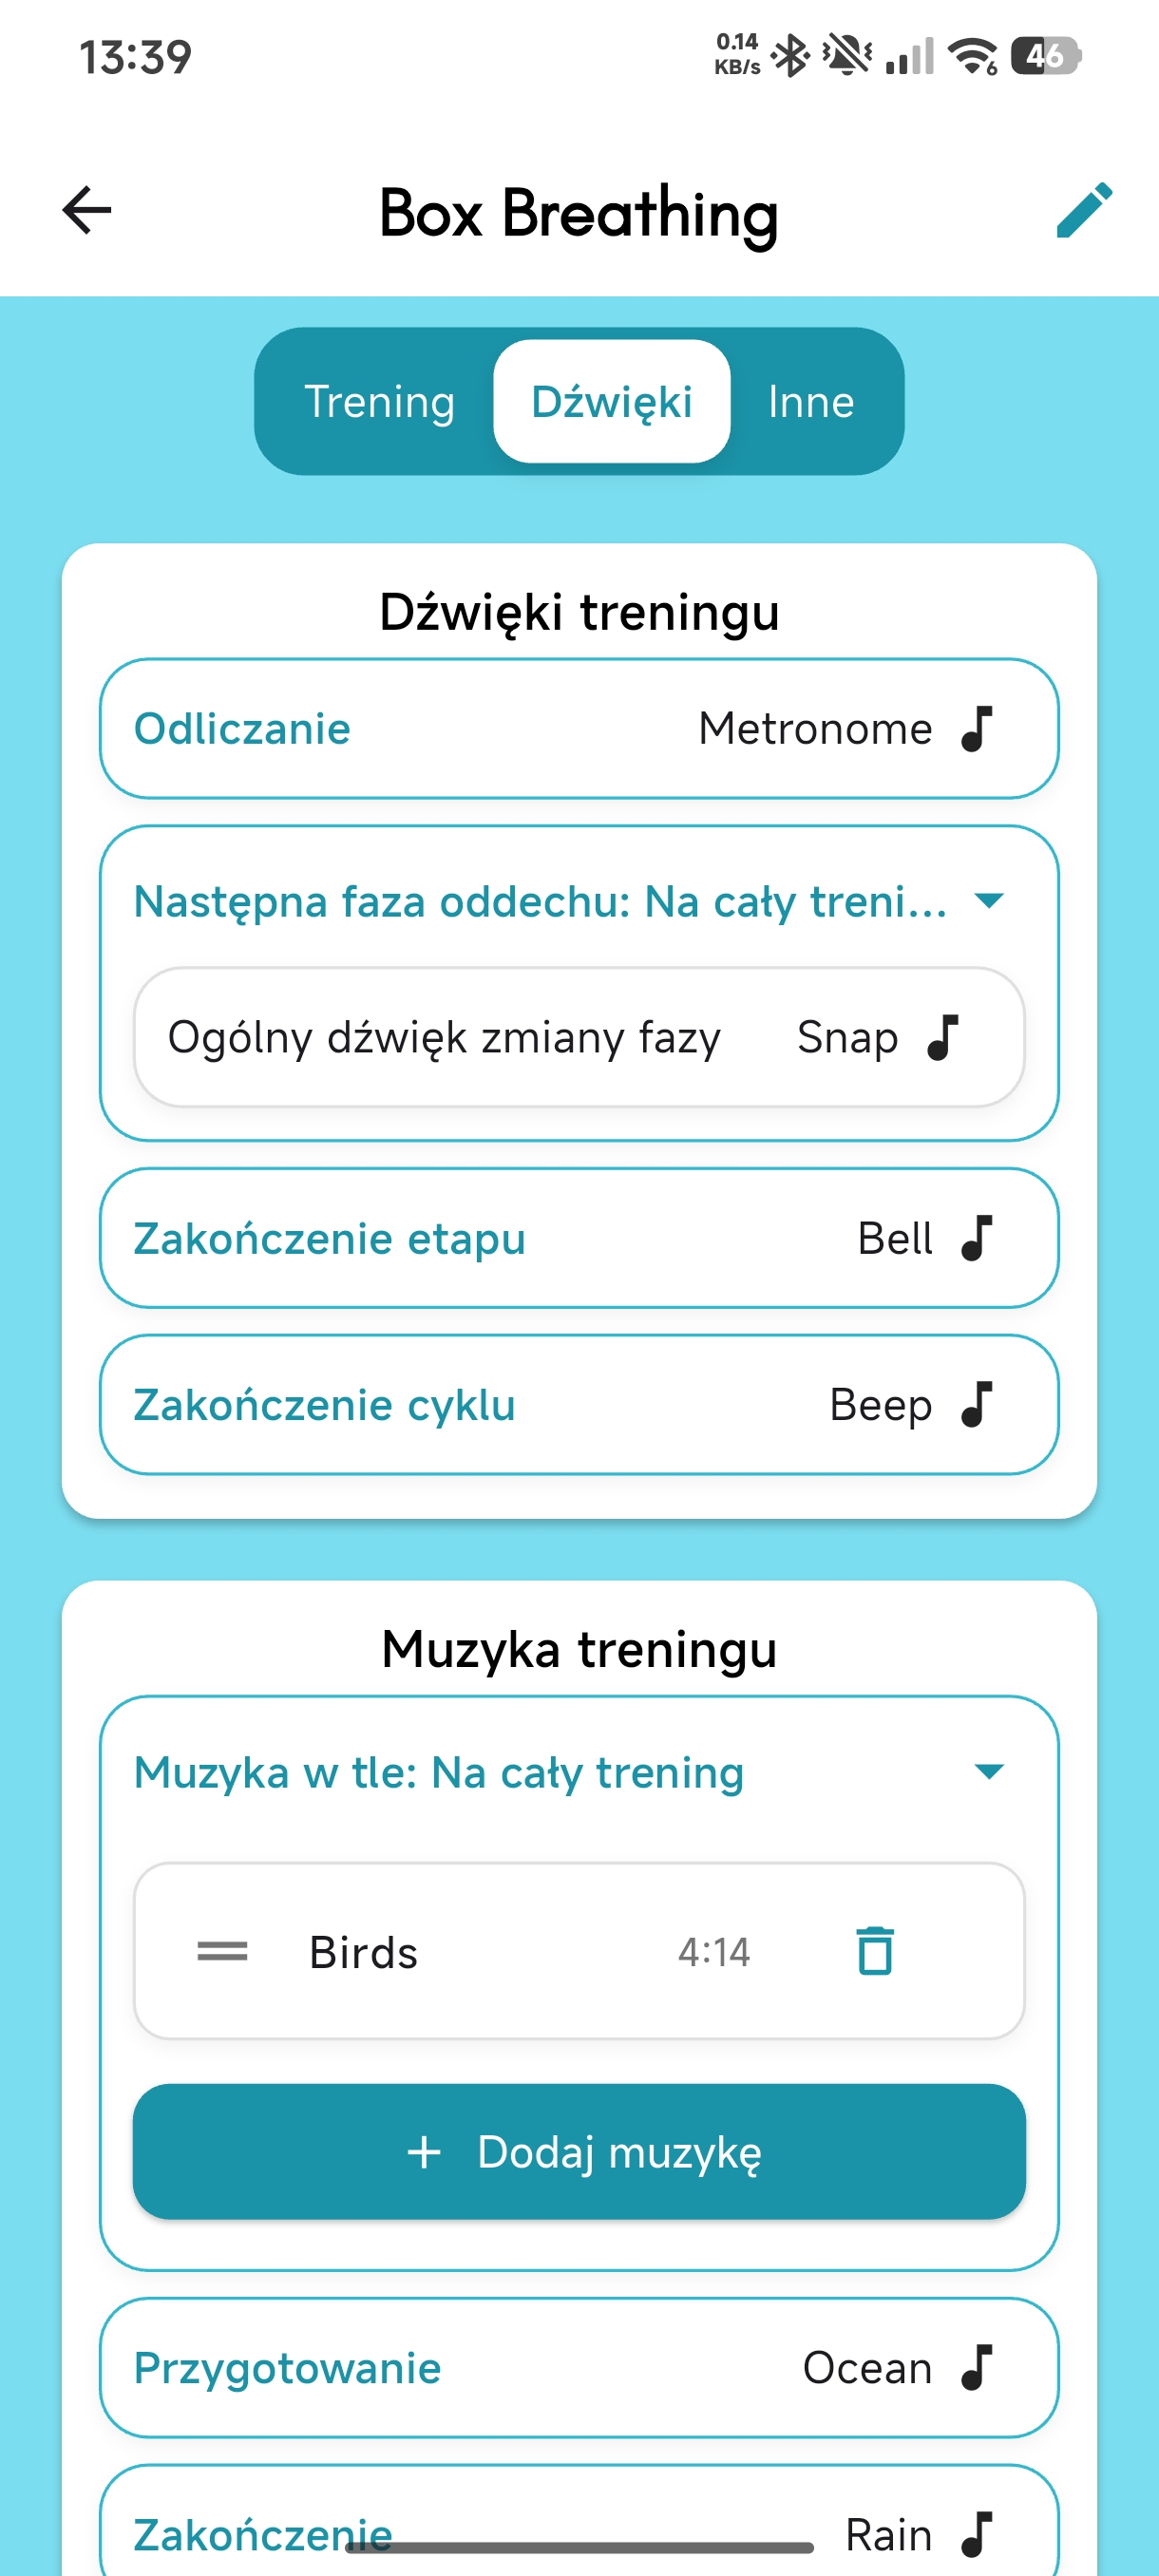
\includegraphics[width=\dimexpr\linewidth-2\fboxrule\relax,height=0.62\textheight,keepaspectratio]{obrazy/badania_interface/sound_settings_old_music.jpg}}}
        \par\small (a)
    \end{minipage}\hfill
    \begin{minipage}[c]{0.08\linewidth}
        \centering
        {\large $\rightarrow$}
    \end{minipage}\hfill
    \begin{minipage}[c]{0.44\linewidth}
        \centering
        {\setlength{\fboxsep}{0pt}\setlength{\fboxrule}{0.2pt}\fcolorbox{gray}{white}{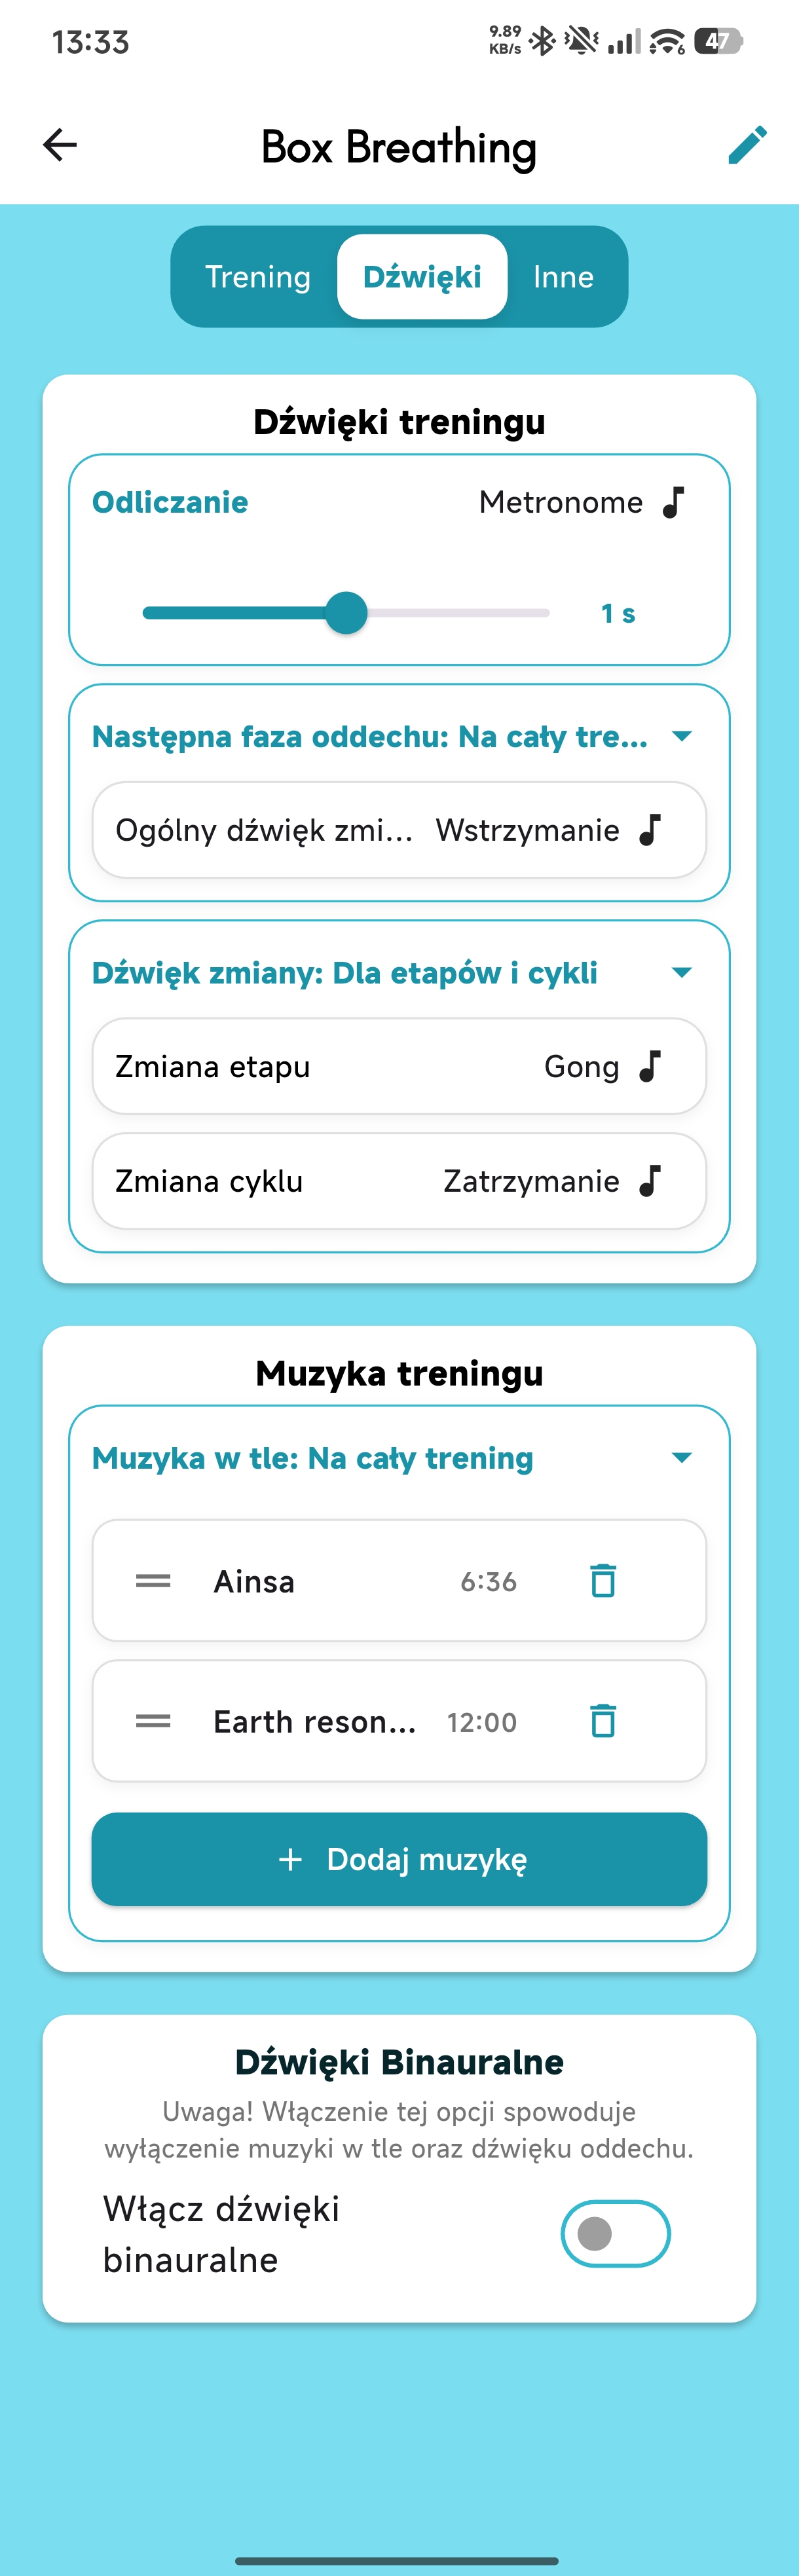
\includegraphics[width=\dimexpr\linewidth-2\fboxrule\relax,height=0.62\textheight,keepaspectratio]{obrazy/badania_interface/sounds_settings_new_music.jpg}}}
        \par\small (b)
    \end{minipage}
    \caption[Ustawienia muzyki i sygnałów dźwiękowych przed zmianami i po reorganizacji]{Ustawienia muzyki i sygnałów dźwiękowych: (a) ekran przed zmianami; (b) ekran po ujednoliceniu komponentów i reorganizacji ustawień}
    \label{fig:ux_music_settings}
\end{figure}

Zmieniono również sposób konfiguracji dźwięków binauralnych. Zamiast niezależnie ustawiać częstotliwość dla lewego i prawego ucha, użytkownik wybiera częstotliwość bazową oraz różnicę częstotliwości. Ekran wskazuje kategorię odpowiadającą wybranej różnicy zgodnej z częstotliwościami Solfeggio, na przykład alpha, beta lub gamma. Są to dźwięki, które mogą w różny sposób wpływać na doświadczenia użytkownika podczas sesji ćwiczeń oddechu. Odpowiednie konfiguracje mogą pomóc w zrelaksowaniu się lub pobudzeniu organizmu. Nowy interfejs pozwala dobierać ustawienie bez samodzielnego obliczania różnicy pomiędzy kanałami. Oba warianty konfiguracji przedstawiono na rysunku \ref{fig:ux_binaural_settings}.

W aplikacji muzyka w tle oraz dźwięki binauralne są trybami wzajemnie wykluczającymi się. Aktywowanie dźwięków binauralnych wymaga wyłączenia muzyki, natomiast uruchomienie muzyki wyklucza jednoczesne korzystanie z dźwięków binauralnych.

\begin{figure}[H]
    \centering
    \begin{minipage}[c]{0.44\linewidth}
        \centering
        {\setlength{\fboxsep}{0pt}\setlength{\fboxrule}{0.2pt}\fcolorbox{gray}{white}{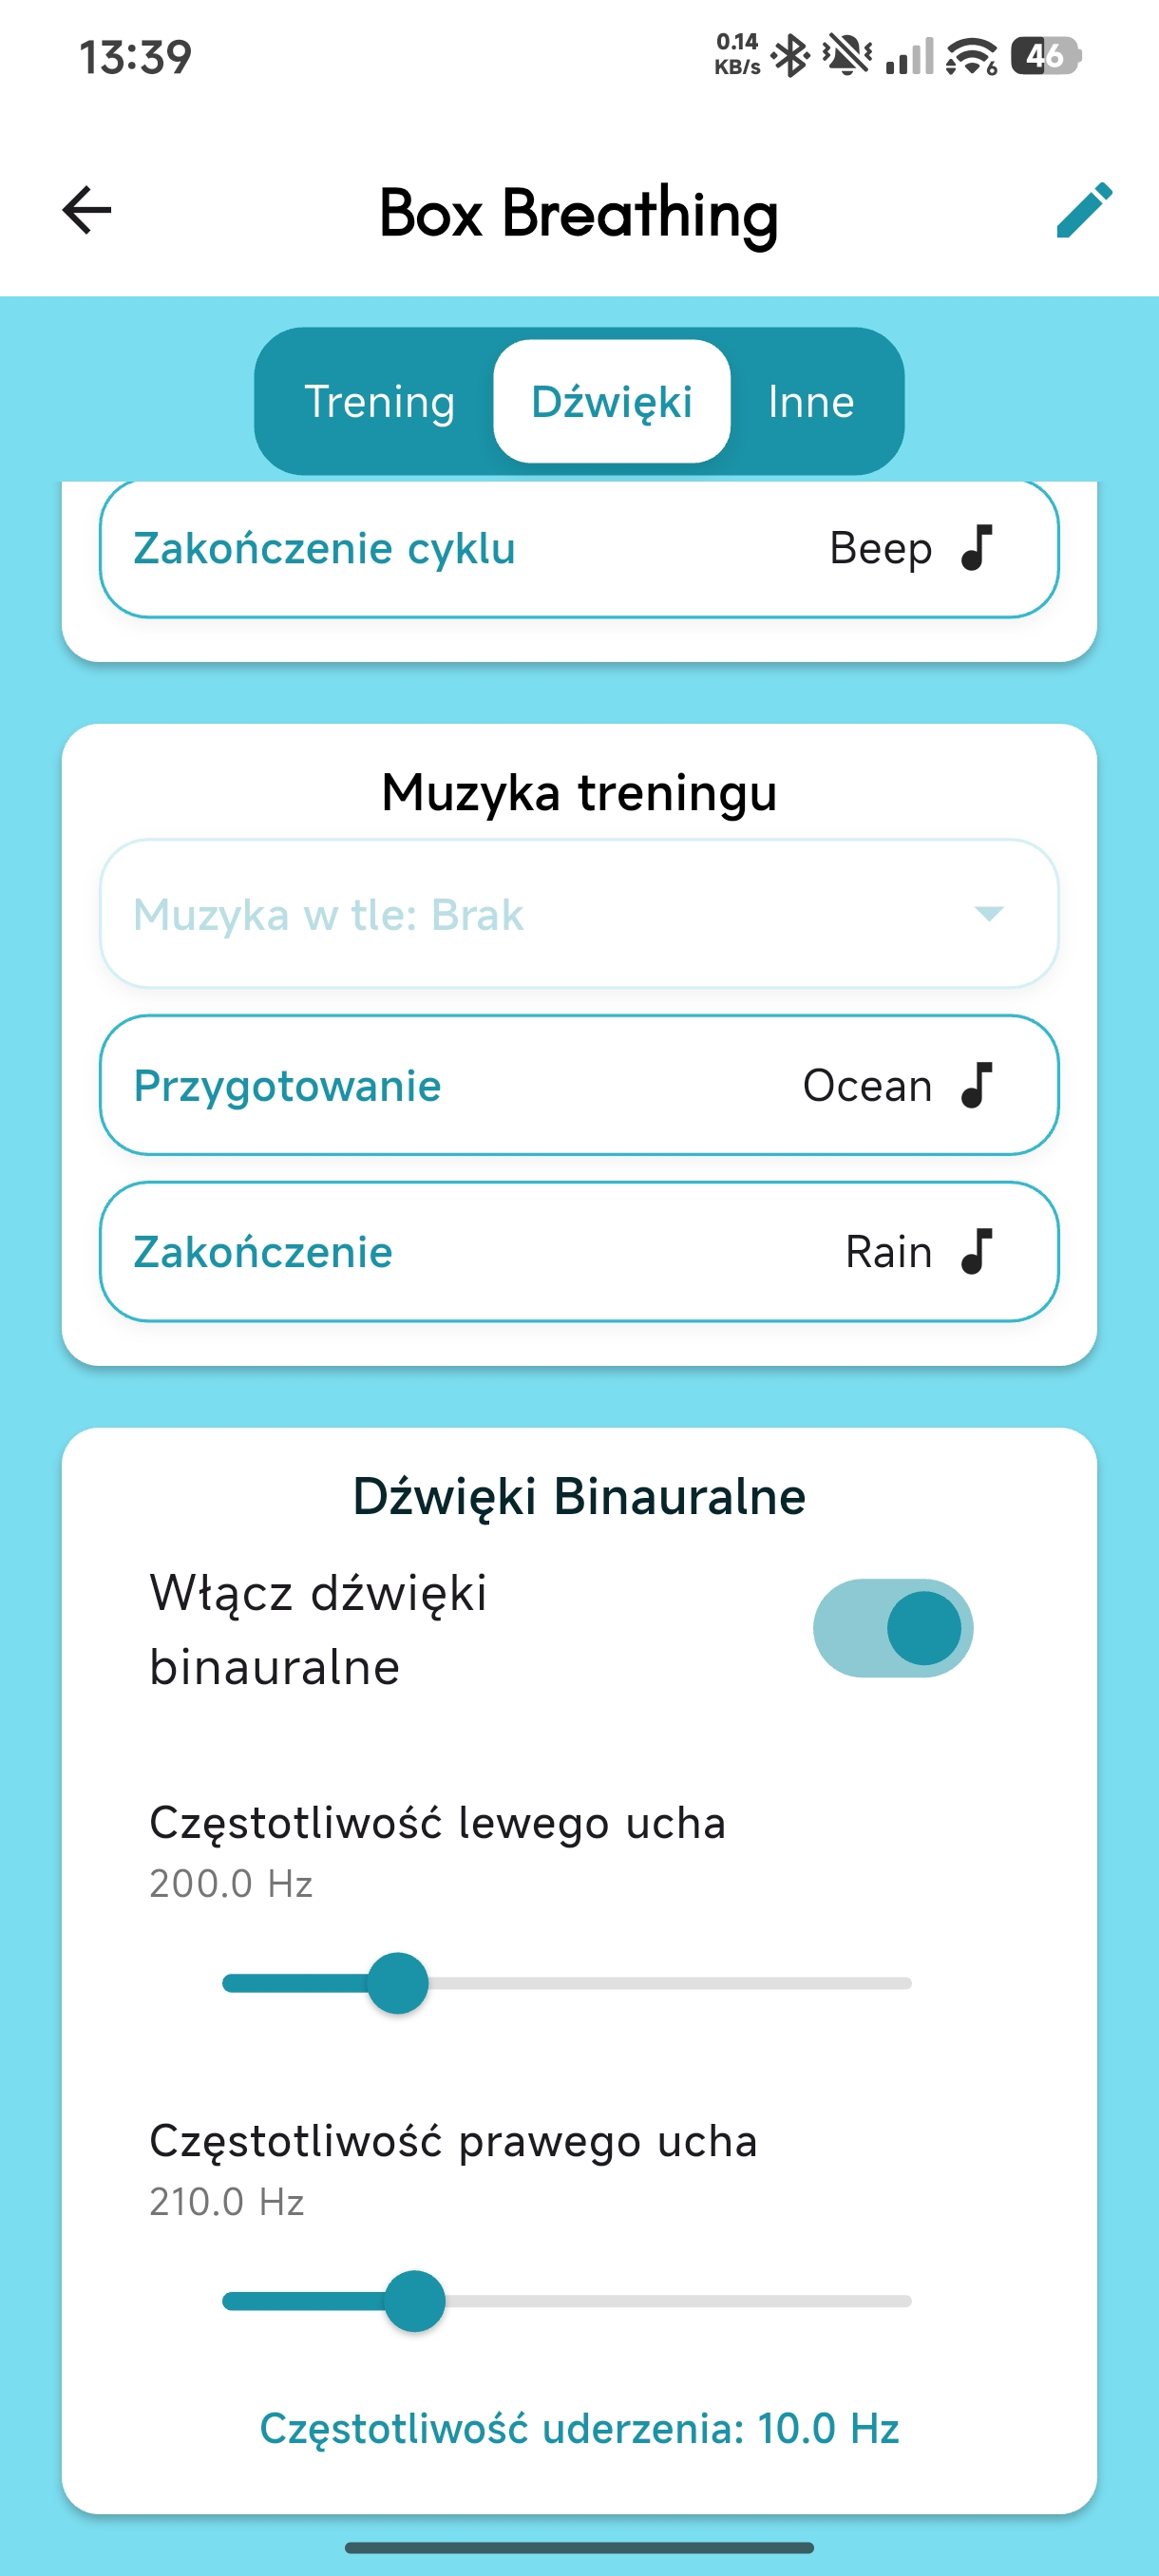
\includegraphics[width=\dimexpr\linewidth-2\fboxrule\relax,height=0.57\textheight,keepaspectratio]{obrazy/badania_interface/sound_settings_old_binaural.jpg}}}
        \par\small (a)
    \end{minipage}\hfill
    \begin{minipage}[c]{0.08\linewidth}
        \centering
        {\large $\rightarrow$}
    \end{minipage}\hfill
    \begin{minipage}[c]{0.44\linewidth}
        \centering
        {\setlength{\fboxsep}{0pt}\setlength{\fboxrule}{0.2pt}\fcolorbox{gray}{white}{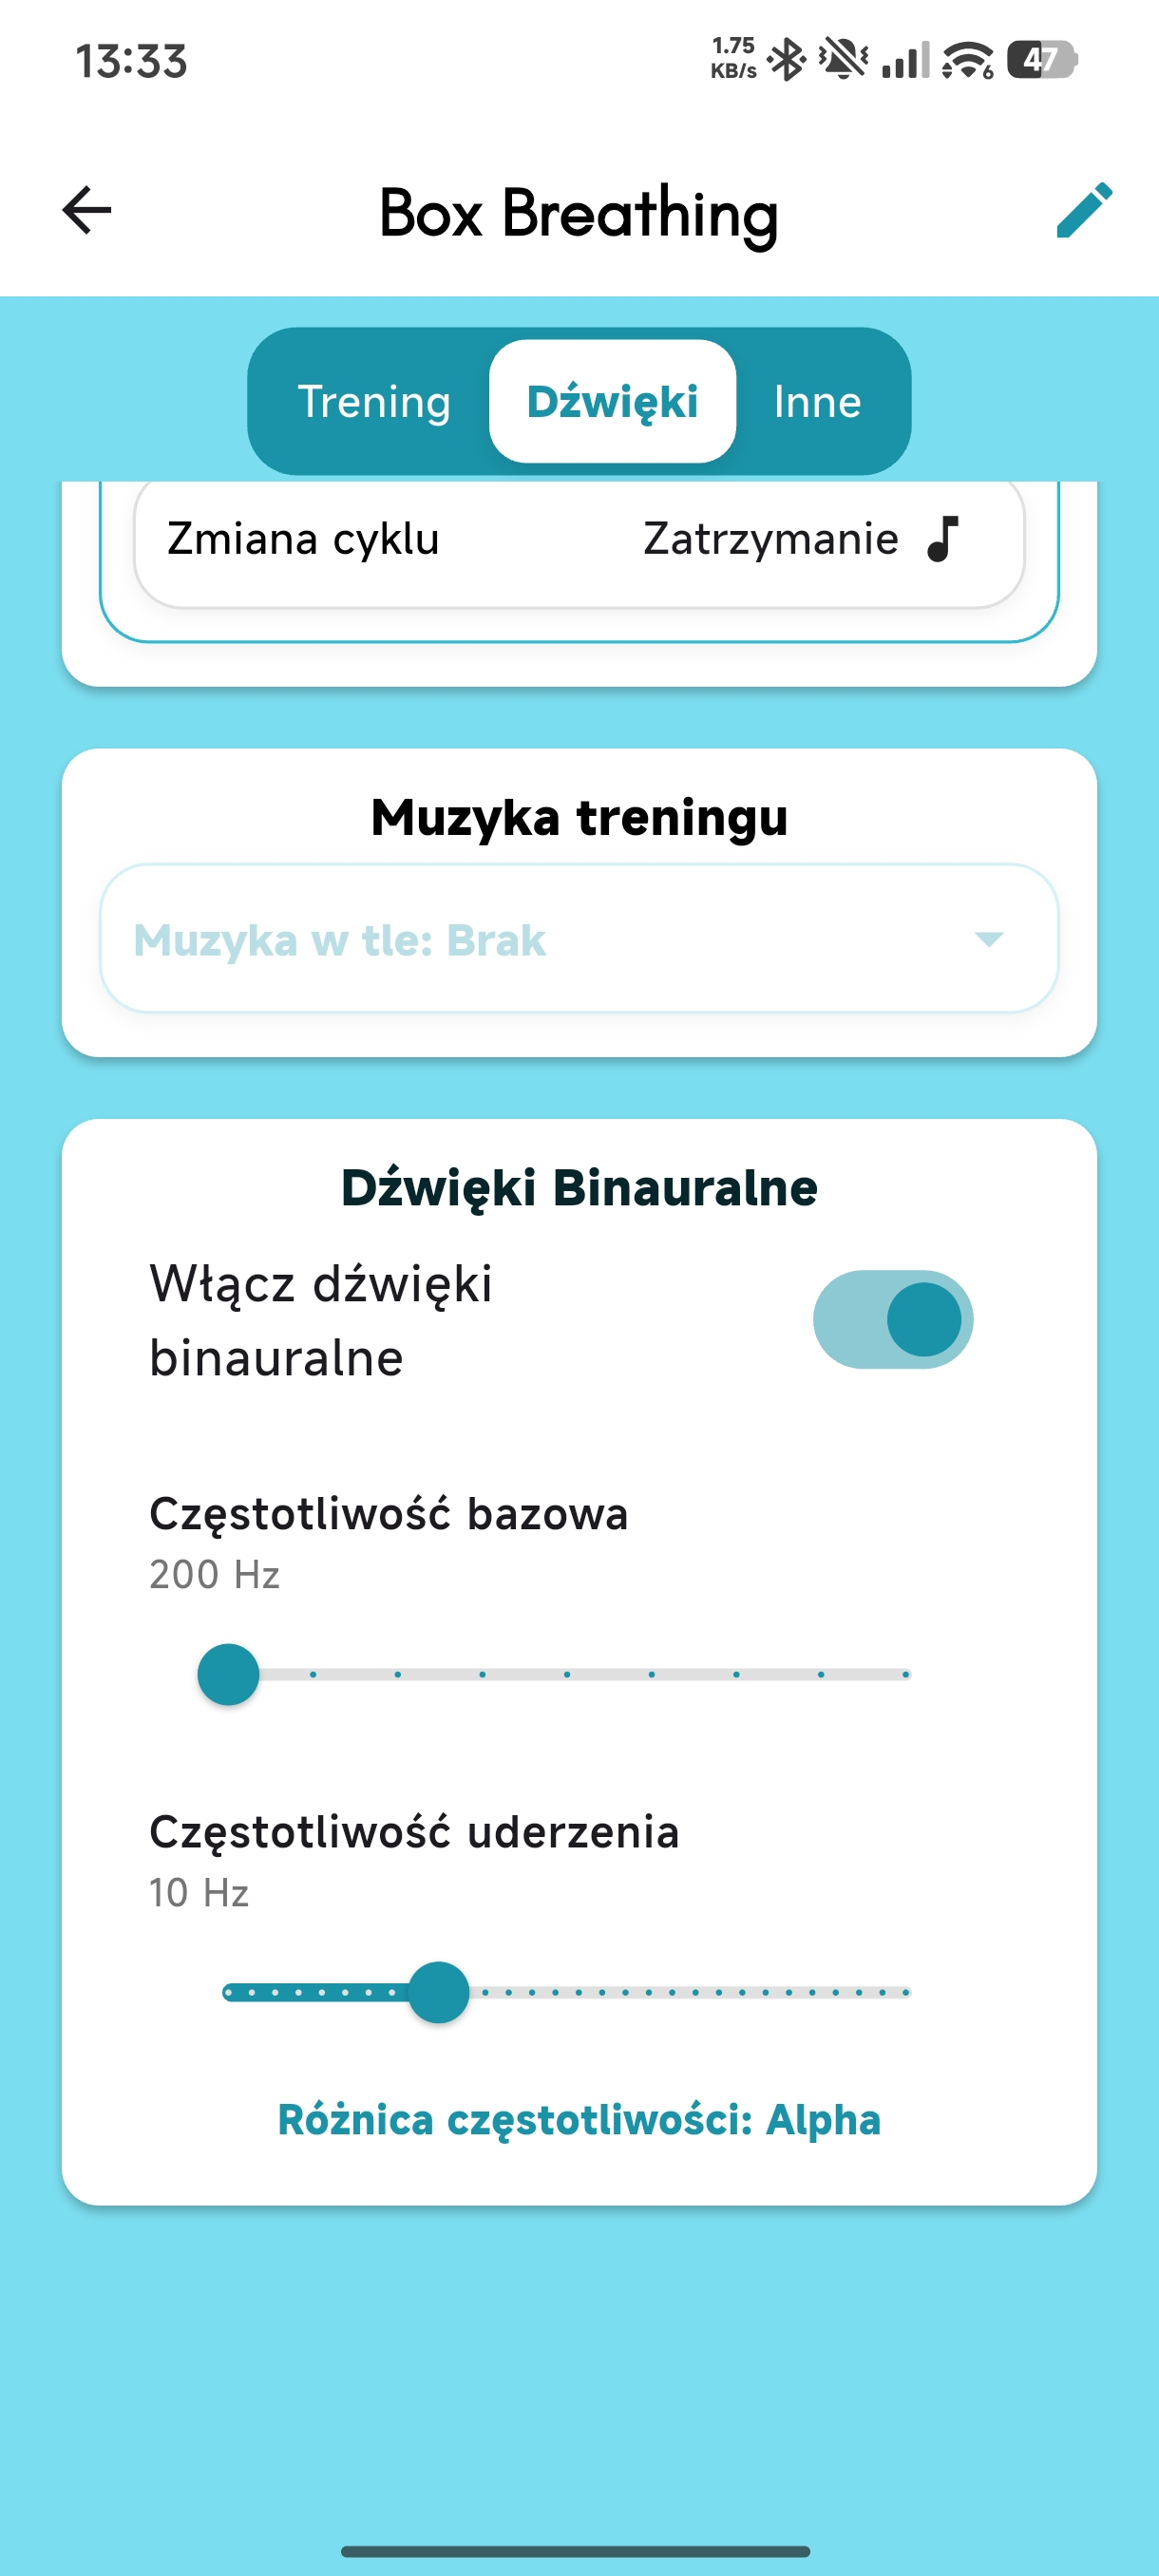
\includegraphics[width=\dimexpr\linewidth-2\fboxrule\relax,height=0.57\textheight,keepaspectratio]{obrazy/badania_interface/sounds_settings_new_binaural.jpg}}}
        \par\small (b)
    \end{minipage}
    \caption[Zmiana sposobu konfiguracji dźwięków binauralnych]{Konfiguracja dźwięków binauralnych: (a) niezależne ustawianie częstotliwości kanałów przed zmianami; (b) wybór częstotliwości bazowej i różnicy częstotliwości po zmianach}
    \label{fig:ux_binaural_settings}
\end{figure}

\subsection{Pozostałe ustawienia treningu}

Zakładkę \textit{Inne} rozszerzono o opcję wygaszania ekranu podczas treningu prowadzonego wyłącznie za pomocą wskazówek dźwiękowych. Użytkownik może określić czas, po którym ekran zostanie wygaszony. Umożliwia to kontynuowanie ćwiczenia bez stałego wyświetlania animacji. W tej samej zakładce umieszczono przełącznik zliczania cykli oddechowych na podstawie sygnału z mikrofonu, dzięki któremu można włączyć lub wyłączyć monitorowanie oddechu.

W dolnej części ekranu dodano wybór stylu wizualizacji opisanego w podrozdziale \ref{sec:ux_breathing_visualization}. Dla widoku osi czasu dostępna jest dodatkowo sonifikacja wskazówek oddechowych. Jej włączenie wyłącza dźwięki binauralne, co zapobiega jednoczesnemu uruchomieniu tych dwóch trybów dźwiękowych. Porównanie zawartości zakładki przed rozbudową i po niej przedstawiono na rysunku \ref{fig:ux_other_settings}.

\begin{figure}[H]
    \centering
    \begin{minipage}[c]{0.44\linewidth}
        \centering
        {\setlength{\fboxsep}{0pt}\setlength{\fboxrule}{0.2pt}\fcolorbox{gray}{white}{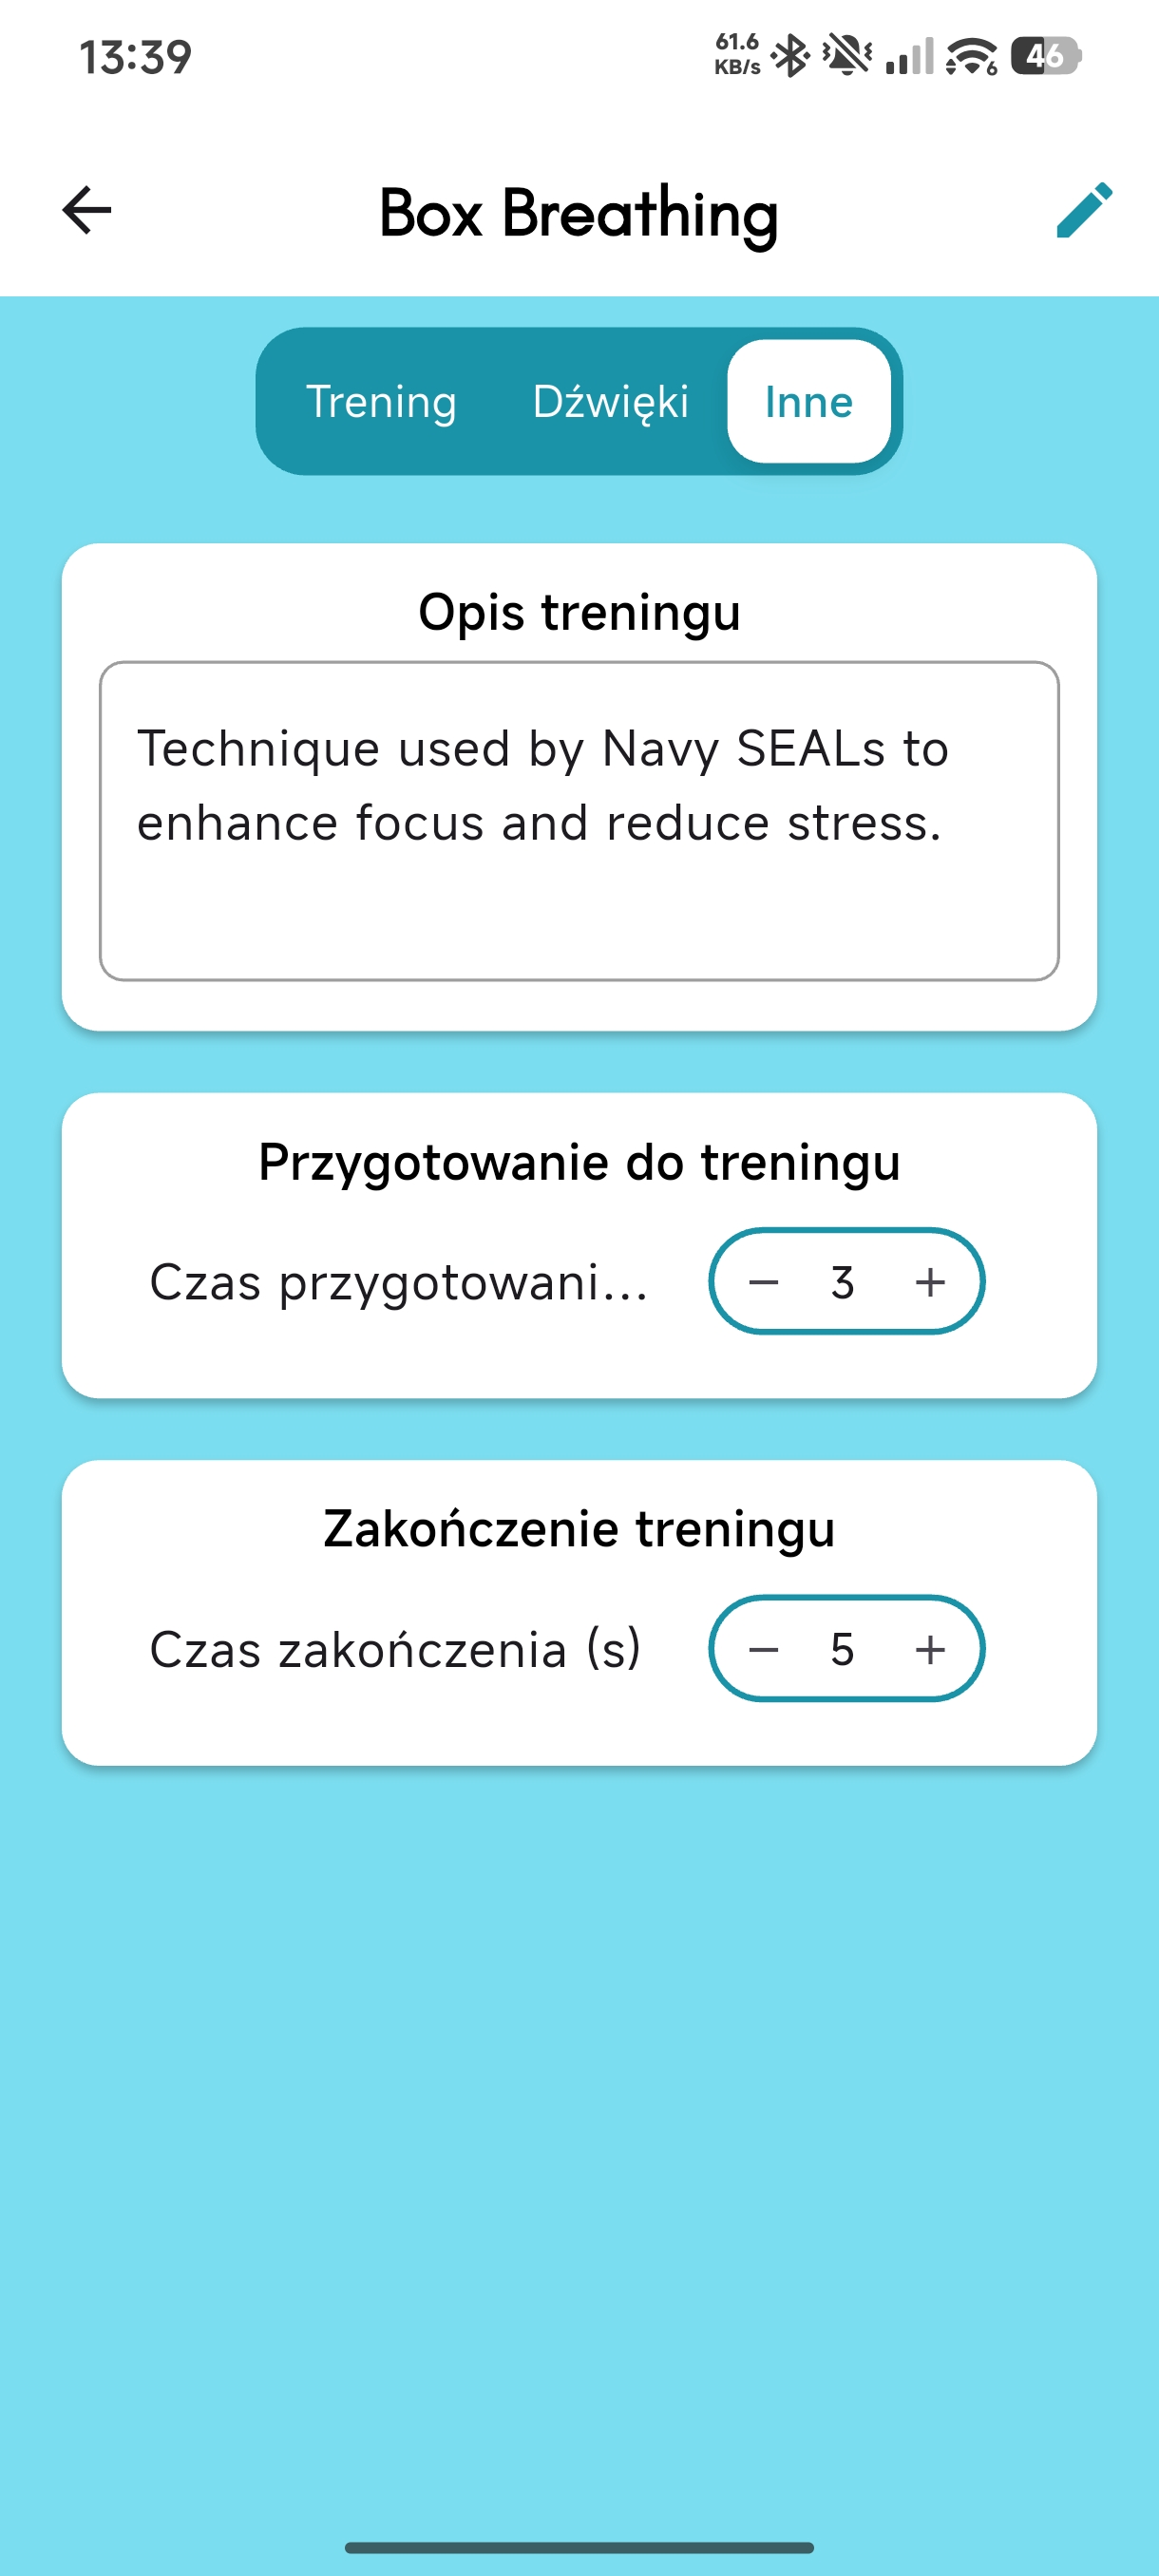
\includegraphics[width=\dimexpr\linewidth-2\fboxrule\relax,height=0.64\textheight,keepaspectratio]{obrazy/badania_interface/other_settings_old.jpg}}}
        \par\small (a)
    \end{minipage}\hfill
    \begin{minipage}[c]{0.08\linewidth}
        \centering
        {\large $\rightarrow$}
    \end{minipage}\hfill
    \begin{minipage}[c]{0.44\linewidth}
        \centering
        {\setlength{\fboxsep}{0pt}\setlength{\fboxrule}{0.2pt}\fcolorbox{gray}{white}{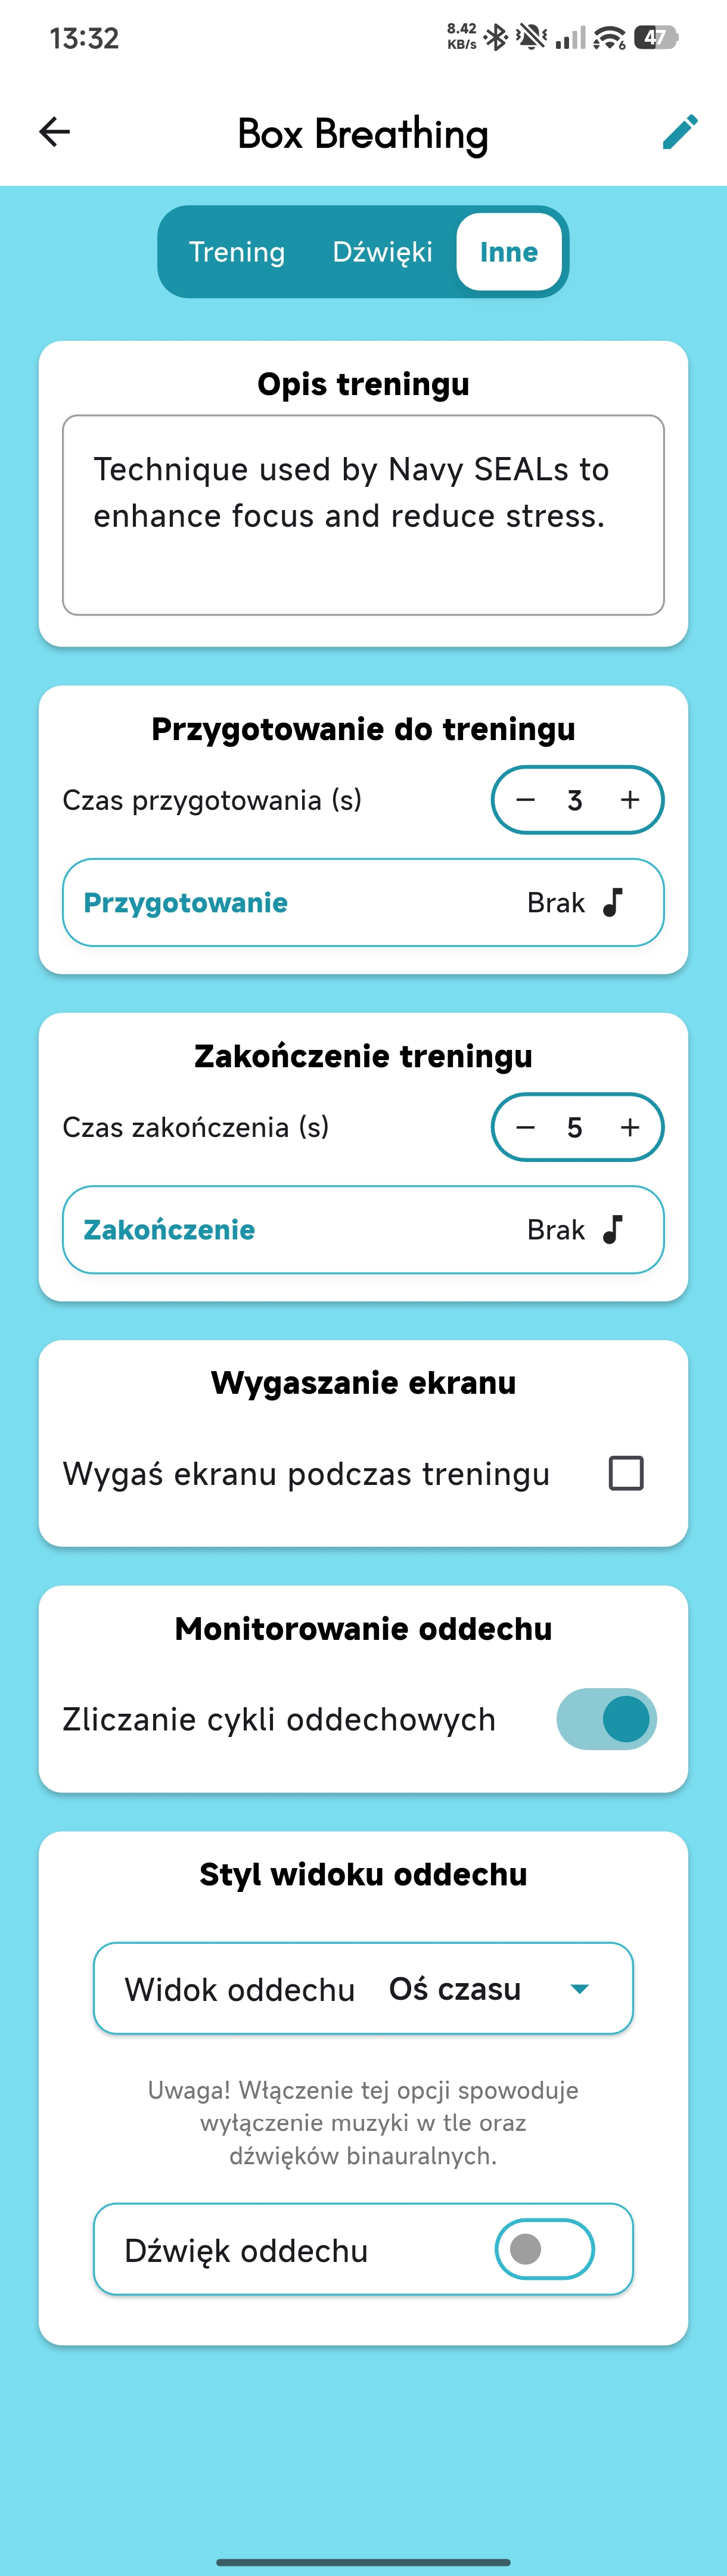
\includegraphics[width=\dimexpr\linewidth-2\fboxrule\relax,height=0.64\textheight,keepaspectratio]{obrazy/badania_interface/other_settings_new.jpg}}}
        \par\small (b)
    \end{minipage}
    \caption[Zakładka Inne przed zmianami i po rozbudowie]{Zakładka Inne: (a) ekran przed zmianami; (b) ekran po dodaniu wygaszania ekranu, monitorowania oddechu i wyboru wizualizacji}
    \label{fig:ux_other_settings}
\end{figure}

\subsection{Kalibracja detekcji wydechu do używanego sprzętu}

Dodano ekran umożliwiający dostosowanie czułości wykrywania wydechu. Użytkownik może zmienić jej wartość za pomocą suwaka, uruchomić test mikrofonu i sprawdzić reakcję detektora na wykonywany wydech. Pozwala to dobrać ustawienie do używanego telefonu oraz zestawu słuchawkowego bez zmiany wag modelu ani ponownego uczenia sieci. Czułość prezentowana w interfejsie nie jest standardowym progiem prawdopodobieństwa klasy \textit{Exhale}: jej zwiększenie ułatwia przypisanie próbki do tej klasy, a więc może zwiększyć zarówno liczbę poprawnych, jak i fałszywych detekcji.

Połączenie regulacji czułości z możliwością bezpośredniego testowania zapewnia informację zwrotną podczas konfiguracji. Użytkownik może sprawdzić, czy wydechy są wykrywane oraz czy detektor reaguje także na inne dźwięki, a następnie skorygować ustawienie. Ekran przedstawiono na rysunku \ref{fig:ux_threshold_tester}. Wyniki doboru czułości w testowanych konfiguracjach sprzętowych omówiono w~dalszej części rozdziału, w podrozdziale dotyczącym testów na urządzeniach mobilnych.

\begin{figure}[H]
    \centering
    {\setlength{\fboxsep}{0pt}\setlength{\fboxrule}{0.2pt}\fcolorbox{gray}{white}{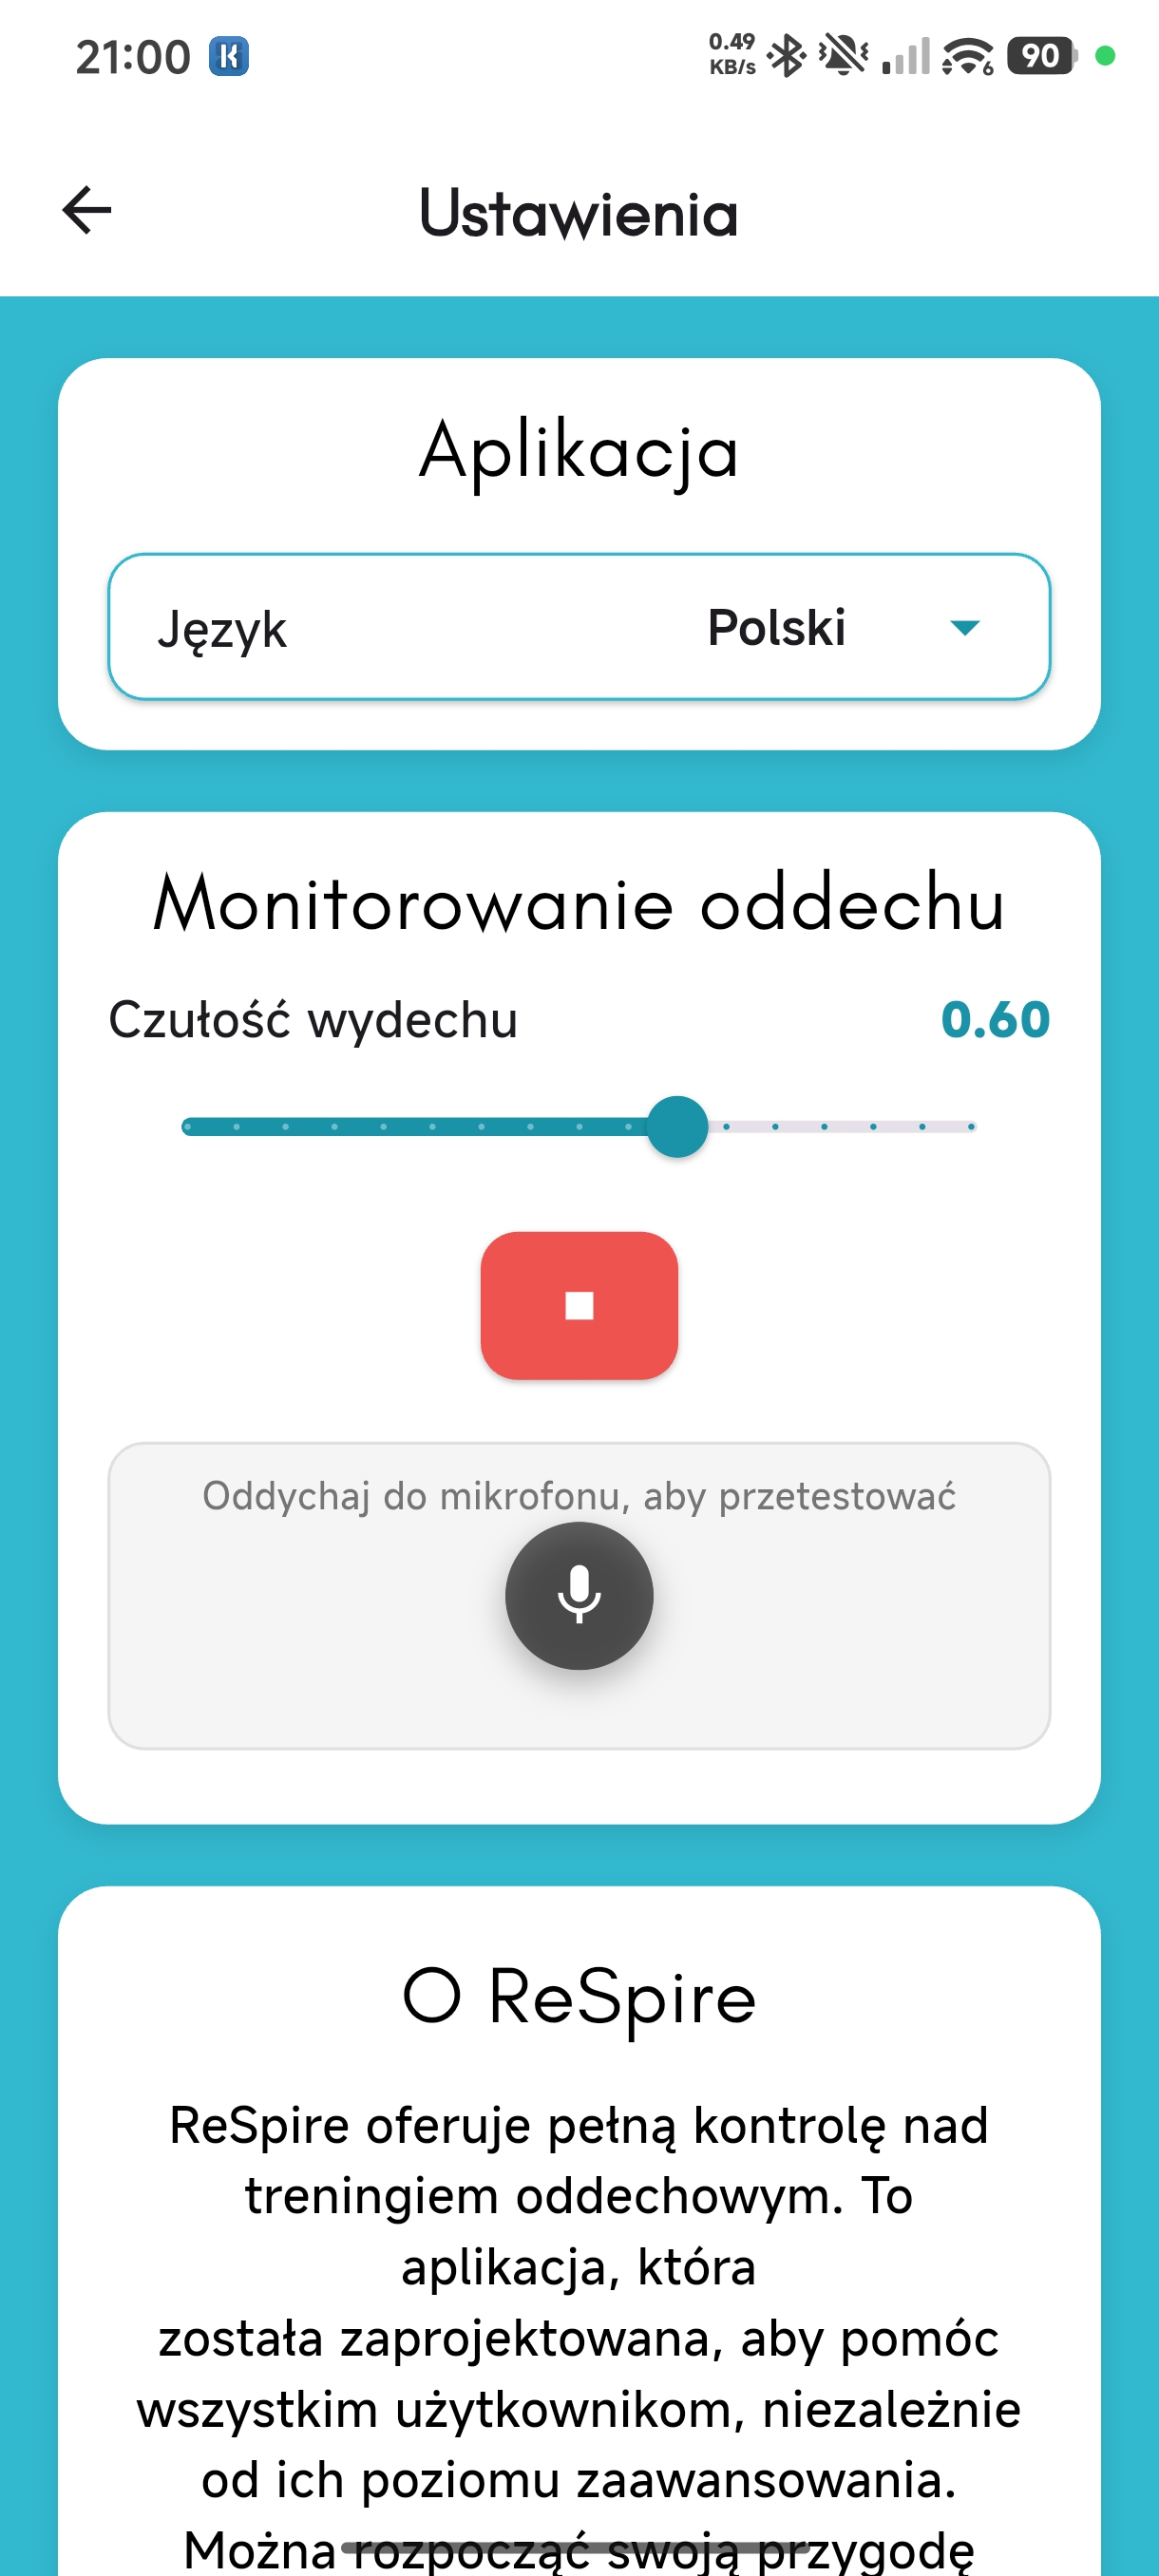
\includegraphics[width=0.43\linewidth,height=0.60\textheight,keepaspectratio]{obrazy/badania_interface/treshold_tester_new.jpg}}}
    \caption{Ekran regulacji czułości i testowania detekcji wydechu z użyciem mikrofonu}
    \label{fig:ux_threshold_tester}
\end{figure}

\section{Usprawnienie działania modelu wykrywania wydechu}

W ramach rozwoju systemu porównano dwie wersje modelu wykrywania wydechu. Model \textit{breathing classification v2} (BCV2) stanowił punkt odniesienia. Udoskonalony model \textit{breathing classification v3} (BCV3) został wytrenowany na rozszerzonym zbiorze danych oraz uzupełniony o mechanizmy ograniczające przeuczenie i wpływ nierównomiernego rozkładu klas. Oba modele oceniono na tym samym zbiorze testowym zawierającym 11~705 próbek dźwięku, w tym 7206 przykładów klasy \textit{Exhale} oraz 4499 przykładów klasy \textit{Other}.

\subsection{Dodatkowe dane}

Podstawowym usprawnieniem BCV3 było zwiększenie liczby danych wykorzystanych podczas uczenia. Większy zbiór zawierał więcej przykładów zróżnicowanych sposobów wykonywania wydechu, a także próbek należących do klasy \textit{Other}. Pozwoliło to modelowi poznać szerszy zakres cech występujących w sygnale i ograniczyć dopasowanie do niewielkiej liczby nagrań. Zwiększenie różnorodności danych jest szczególnie istotne w aplikacji mobilnej, ponieważ natężenie oraz charakter dźwięku oddechu zależą między innymi od użytkownika, odległości od mikrofonu, jak również warunków otoczenia.

\subsection{Dostosowanie architektury}

W architekturze BCV3 dodano warstwy dropout. Podczas treningu losowo wyłączają one część aktywacji, przez co sieć nie może nadmiernie uzależniać predykcji od pojedynczych cech. Rozwiązanie to pełni funkcję regularyzacji i zmniejsza ryzyko przeuczenia, poprawiając zdolność modelu do działania na nagraniach niewykorzystywanych podczas uczenia.

Drugą zmianą było zastosowanie ważonej funkcji straty (ang. \textit{weighted loss}). Klasy w zbiorze treningowym nie były reprezentowane równomiernie, dlatego ich wagi wyznaczono na podstawie udziału poszczególnych klas w danych. Klasa występująca rzadziej otrzymała większą wagę, natomiast częstsza mniejszą. Dzięki temu błąd popełniony dla mniej licznej klasy miał większy wpływ na aktualizację parametrów modelu. Ograniczyło to tendencję sieci do preferowania klasy dominującej oraz pozwoliło uzyskać bardziej zrównoważone wyniki.

\subsection{Porównanie wyników}

Model zwraca dla analizowanego fragmentu dźwięku wartość interpretowaną jako prawdopodobieństwo przynależności do klasy \textit{Exhale}. Próg decyzyjny $\theta$ określa minimalną wartość wymaganą do wykrycia wydechu:

\begin{equation}
    \widehat{y} = \begin{cases}
        \textit{Exhale}, & p(\textit{Exhale}) \geq \theta, \\
        \textit{Other}, & p(\textit{Exhale}) < \theta.
    \end{cases}
\end{equation}

Przykładowo wynik $p(\textit{Exhale})=0{,}62$ zostanie uznany za wydech przy progu 0,5 lub 0,6, ale nie przy progu 0,7. Zwiększenie progu powoduje więc przypisywanie mniejszej liczby próbek do klasy \textit{Exhale}. W konsekwencji maleją wartości TP i FP, natomiast rosną TN i FN.

Badania przeprowadzono dla progów od 0,3 do 0,7. Próg wybierano przez maksymalizację dokładności na zbiorze testowym, zgodnie ze wzorem $\mathrm{Accuracy}=(TP+TN)/(TP+TN+FP+FN)$. Dla BCV3 w formacie ONNX najwyższą wartość uzyskano przy progu 0,5 czyli $89\%$. Nie maksymalizowano osobno czułości ani wyniku F1 klasy \textit{Exhale}. Wybrany został próg zapewniający największy udział wszystkich poprawnych klasyfikacji.

Analiza kilku progów była istotna również ze względu na różnice pomiędzy mikrofonami urządzeń mobilnych. Poszczególne telefony mogą rejestrować dźwięk z inną czułością, poziomem wzmocnienia i charakterystyką szumów, co wpływa na wartości zwracane przez model. Jeden stały próg nie musi zatem zapewniać równie dobrej detekcji na każdym urządzeniu. Z tego względu aplikacja umożliwia regulację odpowiadającej mu czułości bez modyfikowania ani ponownego trenowania modelu.

\begin{table}[htbp]
    \centering
    \caption{Porównanie modeli ONNX dla progu decyzyjnego 0,5}
    \label{tab:model_versions_comparison}
    \scriptsize
    \setlength{\tabcolsep}{4pt}
    \renewcommand{\arraystretch}{1.2}
    \begin{tabular}{@{}lrrrrrr@{}}
        \toprule
        \textbf{Wariant} & \textbf{Dokł.} & \textbf{Prec. E} & \textbf{Czuł. E} & \textbf{F1 E} & \textbf{F1 macro} & \textbf{ROC-AUC} \\
        \midrule
        BCV3 & \textbf{85,89\%} & 84,43\% & \textbf{94,52\%} & \textbf{89,19\%} & \textbf{84,45\%} & 90,19\% \\
        BCV2 & 84,95\% & \textbf{84,80\%} & 92,05\% & 88,28\% & 83,63\% & \textbf{91,56\%} \\
        \bottomrule
    \end{tabular}
\end{table}

BCV3 w formacie ONNX osiągnął dokładność 85,89\%, czyli o 0,94 punktu procentowego więcej od BCV2 przy tym samym progu. Wynik F1 dla klasy \textit{Exhale} wzrósł z 88,28\% do 89,19\%, a jej czułość z 92,05\% do 94,52\%. Wysoka czułość jest istotna z punktu widzenia aplikacji, ponieważ pominięcie wydechu może spowodować niezliczenie wykonanego cyklu oddechowego.

Macierz pomyłek wersji ONNX pokazuje, że przy progu 0,5 BCV3 prawidłowo rozpoznał 6811 z 7206 próbek wydechu, podczas gdy BCV2 rozpoznał ich 6633. Liczba pominiętych wydechów zmniejszyła się z 573 do 395. Jednocześnie liczba próbek klasy \textit{Other} błędnie uznanych za wydech wzrosła z 1189 do 1256. BCV3 przesuwa zatem punkt pracy w stronę większej czułości, co jest korzystne dla zliczania cykli, lecz wymaga uwzględnienia ryzyka dodatkowych fałszywych detekcji.

BCV2 uzyskał nieznacznie wyższy wynik ROC-AUC: 0,9156 w porównaniu z 0,9019 dla BCV3. Oznacza to, że przewaga BCV3 nie występuje dla każdej możliwej wartości progu. Przy przyjętym progu 0,5 BCV3 zapewnia jednak wyższą dokładność, czułość i wynik F1 dla wydechu, dlatego został uznany za lepiej dostosowany do docelowego zastosowania w aplikacji.

\subsection{Macierze pomyłek}

Macierze pomyłek modeli ONNX przeanalizowano dla wszystkich badanych wartości progu. W tabeli \ref{tab:all_confusion_matrices} zastosowano standardowe oznaczenia: TP (ang. \textit{true positive}) oznacza poprawnie wykryty wydech, TN (ang. \textit{true negative}) - poprawnie rozpoznana próbka klasy \textit{Other}, FP (ang. \textit{false positive}) - próbka klasy \textit{Other} błędnie uznany za wydech, natomiast FN (ang. \textit{false negative}) - pominięty wydech.

\begin{table}[htbp]
    \centering
    \caption{Porównanie macierzy pomyłek modeli ONNX dla badanych progów decyzyjnych}
    \label{tab:all_confusion_matrices}
    \scriptsize
    \setlength{\tabcolsep}{4pt}
    \renewcommand{\arraystretch}{1.08}
    \begin{tabular}{@{}lrrrrrr@{}}
        \toprule
        \textbf{Wariant} & \textbf{Próg} & \textbf{TP} & \textbf{TN} & \textbf{FP} & \textbf{FN} & \textbf{Dokł.} \\
        \midrule
        BCV3 & 0,7 & 6214 & \textbf{3599} & 900 & \textbf{992} & 83,84\% \\
        & 0,6 & 6586 & 3402 & 1097 & 620 & 85,33\% \\
        & 0,5 & 6811 & 3243 & 1256 & 395 & \textbf{85,89\%} \\
        & 0,4 & 6932 & 3065 & 1434 & 274 & 85,41\% \\
        & 0,3 & \textbf{7020} & 2837 & \textbf{1662} & 186 & 84,21\% \\
        \midrule
        BCV2 & 0,7 & 6346 & 3535 & 964 & 860 & 84,42\% \\
        & 0,6 & 6502 & 3418 & 1081 & 704 & 84,75\% \\
        & 0,5 & 6633 & 3310 & 1189 & 573 & 84,95\% \\
        & 0,4 & 6755 & 3184 & 1315 & 451 & 84,91\% \\
        & 0,3 & 6871 & 3017 & 1482 & 335 & 84,48\% \\
        \bottomrule
    \end{tabular}
\end{table}

We wszystkich wariantach zwiększanie progu klasy \textit{Exhale} od 0,3 do 0,7 zmniejszało liczbę próbek przypisanych do tej klasy. Dla BCV3 liczba poprawnych detekcji TP spadła z 7020 do 6214, a liczba fałszywych detekcji FP z 1662 do 900. Jednocześnie liczba pominiętych wydechów FN wzrosła ze 186 do 992. Dobór progu stanowi zatem kompromis pomiędzy ograniczaniem fałszywych detekcji a zachowaniem wysokiej czułości wykrywania wydechu.

BCV3 uzyskiwał wyższą dokładność od BCV2 dla progów 0,4, 0,5 i 0,6. Przy skrajnych wartościach 0,3 i 0,7 nieznacznie lepszy był BCV2. Najwyższą dokładność spośród wszystkich konfiguracji, równą 85,89\%, osiągnął BCV3 w formacie ONNX dla progu 0,5. W tym ustawieniu poprawnie wykrył 6811 wydechów, pomijając 395, oraz prawidłowo rozpoznał 3243 próbki klasy \textit{Other}. W porównaniu z BCV2 przy tym samym progu wykrył o 178 wydechów więcej, kosztem 67 dodatkowych fałszywych detekcji.

Najważniejsze macierze dotyczą progu 0,5 i formatu ONNX, ponieważ ten format jest uruchamiany na urządzeniu mobilnym, a wskazany próg zapewnił najwyższą dokładność. Ich bezpośrednie zestawienie przedstawiono na rysunku \ref{fig:model_confusion_matrices}.

\begin{figure}[H]
    \centering
    \begin{minipage}[t]{0.48\linewidth}
        \centering
        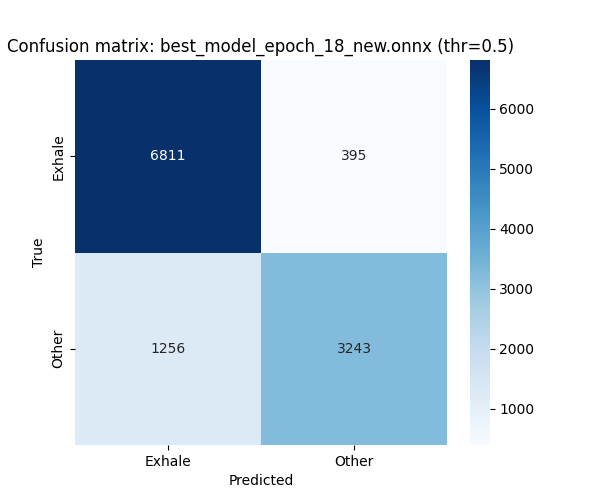
\includegraphics[width=\linewidth]{obrazy/conf_matrix/confusion_best_model_epoch_18_new_onnx_thr_0_5.png}

        \small BCV3
    \end{minipage}
    \hfill
    \begin{minipage}[t]{0.48\linewidth}
        \centering
        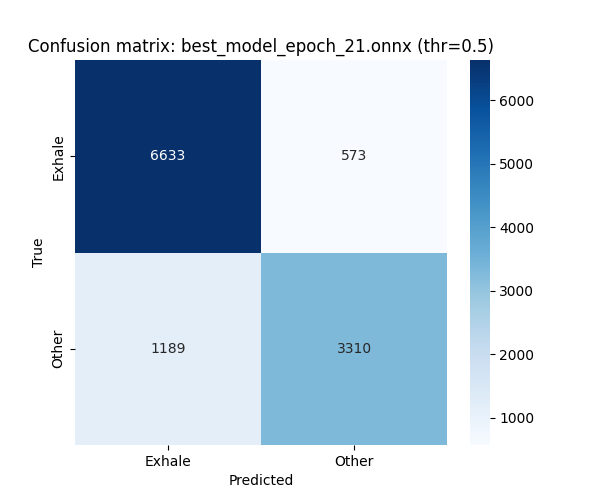
\includegraphics[width=\linewidth]{obrazy/conf_matrix/confusion_best_model_epoch_21_onnx_thr_0_5.png}

        \small BCV2
    \end{minipage}
    \caption{Porównanie macierzy pomyłek modeli BCV3 i BCV2 w formacie ONNX dla progu decyzyjnego 0,5}
    \label{fig:model_confusion_matrices}
\end{figure}

\subsection{Testy na urządzeniach mobilnych}
\subsubsection{Dostosowanie czułości detekcji}
Działanie modelu BCV3 sprawdzono również w warunkach zbliżonych do docelowego wykorzystania aplikacji. Testy przeprowadzono z użyciem emulatora Pixel 3a oraz fizycznych urządzeń Xiaomi Redmi Note 14 Pro i Huawei Mate 20 Lite. Poszczególne konfiguracje różniły się zastosowanym zestawem słuchawkowym, sposobem jego podłączenia oraz dobraną wartością czułości. Zestawienie wykorzystanych konfiguracji przedstawiono w tabeli \ref{tab:mobile_device_thresholds}.

\begin{table}[htbp]
    \centering
    \caption{Konfiguracje wykorzystane podczas testowania modelu na urządzeniach mobilnych}
    \label{tab:mobile_device_thresholds}
    \small
    \setlength{\tabcolsep}{5pt}
    \renewcommand{\arraystretch}{1.2}
    \begin{tabularx}{\textwidth}{@{}p{3.4cm}X p{2.7cm}p{2.1cm}@{}}
        \toprule
        \textbf{Urządzenie} & \textbf{Zestaw słuchawkowy} & \textbf{Połączenie} & \textbf{Dobrana czułość} \\
        \midrule
        Emulator (Pixel 3a) & HyperX Cloud Alpha & Mini jack 3{,}5mm & 0,6 \\
        \midrule
        Huawei Mate 20 Lite & HyperX Cloud Alpha & Mini jack 3{,}5mm & 0,6 \\
        \midrule
        Redmi Note 14 Pro & Poly Blackwire 3220 & USB-C & 0,7 \\
        \bottomrule
    \end{tabularx}
\end{table}

W przypadku emulatora Pixel 3a czułość ustawiono na 0,6 przy wykorzystaniu mikrofonu zestawu HyperX Cloud Alpha. Ten sam zestaw i wartość zastosowano podczas testów na urządzeniu Huawei Mate 20 Lite, gdzie słuchawki podłączono przez złącze mini jack. Dla telefonu Xiaomi Redmi Note 14 Pro użyto zestawu Poly Blackwire 3220 podłączonego przez USB-C, a czułość zwiększono do 0,7. W standardowej interpretacji odpowiada to progom klasy \textit{Exhale} równym odpowiednio 0,4 i 0,3.

Wartości dla urządzeń mobilnych dobrano empirycznie za pomocą ekranu testowania mikrofonu. Przed rozpoczęciem właściwego testu użytkownicy samodzielnie wybierali ustawienie czułości, które w ich subiektywnym odczuciu zapewniało najlepsze działanie detekcji. Sprawdzali przy tym, czy wykonywane wydechy są wykrywane oraz czy inne dźwięki nie powodują nadmiarowych wskazań. Nie maksymalizowano w tym przypadku formalnej miary na oznaczonym zbiorze mobilnym, dlatego wartości te określono jako dobraną czułość, a nie matematycznie optymalny próg. Konieczność zastosowania różnych ustawień potwierdza wpływ charakterystyki mikrofonu, sposobu podłączenia oraz toru przetwarzania dźwięku w urządzeniu.

\subsubsection{Testy wykrywania wydechu podczas treningu}

Skuteczność wykrywania wydechu sprawdzono dodatkowo podczas wykonywania ćwiczeń oddechowych przez użytkowników. Badanie przeprowadzono z użyciem zestawów HyperX Cloud Alpha i Poly Blackwire 3220, zarówno w cichym, jak i głośnym otoczeniu. Każdy uczestnik wykonywał cztery rodzaje treningu: sekwencję obejmującą 4~s wdechu, 2~s wstrzymania oddechu oraz 4~s wydechu, a także symetryczne sekwencje wdechu i wydechu trwające odpowiednio 2~s, 1,5~s oraz 1~s. Dla każdej konfiguracji wartością referencyjną było 30 rzeczywistych wydechów. W tabeli \ref{tab:headset_detection_ratio} przedstawiono zagregowane wyniki pięciu uczestników i obu warunków otoczenia.

Do oceny zastosowano współczynnik detekcji DR (ang. \textit{Detection Ratio}), obliczany według wzoru:

\begin{equation}
    \mathrm{DR} = \frac{N_{\mathrm{det}}}{N_{\mathrm{ref}}} \cdot 100\%,
\end{equation}

gdzie $N_{\mathrm{det}}$ oznacza liczbę wykrytych wydechów, a $N_{\mathrm{ref}}$ liczbę rzeczywistych wydechów.

Wartość DR równa 100\% oznacza zgodność liczby detekcji z liczbą rzeczywistych wydechów. Wynik poniżej 100\% wskazuje na pomijanie wydechów, natomiast wynik przekraczający 100\% oznacza występowanie dodatkowych, fałszywych detekcji. Współczynnik ten opisuje zgodność liczby wykryć, ale nie rozstrzyga, czy każda detekcja została czasowo przypisana do właściwego wydechu.

\begin{table}[H]
    \centering
    \caption{Wyniki wykrywania wydechu dla zestawów HyperX Cloud Alpha i Poly Blackwire 3220}
    \label{tab:headset_detection_ratio}
    \small
    \setlength{\tabcolsep}{5pt}
    \renewcommand{\arraystretch}{1.2}
    \begin{tabular}{@{}lrrrr@{}}
        \toprule
        & \multicolumn{2}{c}{\textbf{HyperX}} & \multicolumn{2}{c}{\textbf{Blackwire}} \\
        \midrule
        \textbf{Test} & \textbf{Detekcje} & \textbf{DR} & \textbf{Detekcje} & \textbf{DR} \\
        \midrule
        4-2-4       & 28,7/30 & 95,60\% & 35,5/30 & 118,30\% \\
        2~s           & 29,0/30 & 96,70\% & 28,0/30 & 93,30\% \\
        1,5~s         & 21,0/30 & 70,00\% & 22,0/30 & 73,30\% \\
        1~s           & 5,0/30  & 16,70\% & 6,0/30  & 20,00\% \\
        \bottomrule
    \end{tabular}
\end{table}

Najlepsze wyniki dla zestawu HyperX uzyskano dla wolniejszych sekwencji 4-2-4 oraz 2~s, dla których DR wyniósł odpowiednio 95,60\% i 96,70\%. Zestaw Blackwire osiągnął zbliżony rezultat dla sekwencji 2~s, natomiast w teście 4-2-4 wartość 118,30\% wskazuje na nadmiarowe detekcje. Wraz ze skracaniem faz skuteczność obu konfiguracji wyraźnie malała. Dla sekwencji 1,5~s współczynnik DR osiągnął 70,00\% dla HyperX i 73,30\% dla Blackwire, a dla najszybszej sekwencji 1~s jedynie 16,70\% oraz 20,00\%.

Wyniki wskazują, że obecna wersja modelu lepiej współpracuje z wolniejszymi treningami, w których dźwięk wydechu trwa wystarczająco długo, aby został prawidłowo zarejestrowany i~sklasyfikowany. Krótkie fazy stanowią większe wyzwanie ze względu na ograniczoną liczbę analizowanych fragmentów sygnału oraz niewielkie odstępy między kolejnymi oddechami. Różnice pomiędzy zestawami potwierdzają również znaczenie charakterystyki mikrofonu, a także dobranej czułości detekcji.
